\documentclass[MScCS]{uccthesis}

%%% Additional packages (not supplied by the class) 
\usepackage{algorithm}          % floating environment for pseudocode
\usepackage{algpseudocode}      % pseudocode body
\usepackage{listings}           % real, selectable source listings
\usepackage{tabularx}           % width-controlled tables
\usepackage{xltabular}          % tabularx X columns that break across pages
\usepackage{array}              % extended column specifiers
\usepackage{ragged2e}           % ragged margins that still hyphenate
\usepackage{multirow}           % spanning cells

\renewcommand{\algorithmicrequire}{\textbf{Input:}}
\renewcommand{\algorithmicensure}{\textbf{Output:}}

%%% Listing style.  The class defines no listing style at all, so this only
%%% adds one; it does not override anything.
\lstdefinestyle{thesiscode}{%
   basicstyle=\ttfamily\scriptsize,
   keywordstyle=\bfseries,
   commentstyle=\itshape,
   stringstyle=\ttfamily,
   numbers=left,
   numberstyle=\tiny,
   numbersep=6pt,
   stepnumber=1,
   showstringspaces=false,
   breaklines=true,
   breakatwhitespace=false,
   columns=fullflexible,
   keepspaces=true,
   tabsize=4,
   frame=single,
   framesep=4pt,
   xleftmargin=14pt,
   captionpos=b
}
\lstset{style=thesiscode,language=Python}
\renewcommand{\lstlistingname}{Listing}

\graphicspath{{Figures/}}

%%% Long typewriter strings (Kaggle dataset paths) cannot be broken by TeX and
%%% overrun the right margin.  The class already loads url, so \path{...} can
%%% wrap them; these are the characters after which a break is permitted.  No
%%% hyphen is inserted, so the path is never misread.
\def\UrlBreaks{\do\/\do\-\do\.}
%%% Float placement.  LaTeX defers any float taller than \floatpagefraction
%%% of the text height to a float-only page; at the default 0.5 the attention
%%% block, Algorithm 2 and the literature table each claimed a whole page.
%%% These are placement thresholds only: no margin, font or leading changes.
\renewcommand{\floatpagefraction}{0.80}
\renewcommand{\topfraction}{0.85}
\renewcommand{\bottomfraction}{0.60}
\renewcommand{\textfraction}{0.10}

%%% Last-resort stretch for lines TeX cannot otherwise fit.  This affects only
%%% lines that would be overfull; it changes no margin, font or leading.
\setlength{\emergencystretch}{2em}

%%% Bibliography (biblatex/biber; hardcoded to authoryear by the class) %%%%%%
\addbibresource{thesisbib.bib}

%%% Title page metadata 
\title{Residual-Gated Dual Attention for Real-Time Pothole Detection}
\author{Vinyas Ravi}
\supervisor{Dr. Md Noor-A-Rahim}
\secondreader{Dr. Krishnendu Guha}
\date{\today}

\abstract{%
   Potholes are hard to localise automatically: irregular in geometry, weakly
   bounded, highly variable in apparent scale, and easily confused with
   shadows, patched asphalt and wet road surfaces.  This dissertation presents
   RGDA-YOLOv8m, which inserts Efficient Channel Attention followed by the
   Convolutional Block Attention Module at three multiscale feature-fusion
   stages of the YOLOv8m neck.  The modules are combined with the unmodified
   features through a learnable scalar gate initialised to zero, so the network
   begins fine-tuning as an exact copy of the pretrained detector.  Evaluation
   uses a deduplicated corpus of 926 images and 2,354 annotations built from
   three public Kaggle repositories, from which 1,078 duplicates were removed
   by normalized-pixel nearest-neighbor matching, and compares nine
   configurations.  Across three seeds RGDA-YOLOv8m attains an mAP@0.5 of
   $0.8141 \pm 0.0142$ and an F1 of $0.7708 \pm 0.0121$, exceeding the
   identically trained no-attention baseline in every paired run, for 0.25\%
   additional parameters and 8.1\% of throughput, at 139.9 frames per second.
   Ablation shows that neither module helps alone. Only their combination does.
   Applying the same block to YOLOv11m, whose backbone already contains partial
   self-attention, instead degrades both metrics.  The value of an added
   attention module is therefore a property of the pairing, not of the module.
}

%\dedication{%
%   Your dedication here.
%}

\acknowledgement{%
   I thank my supervisor, Dr Md Noor-A-Rahim, for guidance and encouragement through-out this project and the second reader, Dr. Krishnendu Guha, for their time and comments. I am grateful to the School of Computer Science and Information Technology at University College Cork for the resources that made this work possible and to the maintainers of the UCI Machine Learning Repository for curating the datasets on which this study rests.
}


\renewcommand\addToFrontMatter[0]{%
   \cleardoublepage%
   \addcontentsline{toc}{chapter}{List of Algorithms}%
   \listofalgorithms%
}

\begin{document}

%%%%%%%%%%%%%%%%%%%%%%%
% CHAPTER 1 -- Introduction
%%%%%%%%%%%%%%%%%%%%%%%

\chapter{Introduction}
\label{ch:introduction}

\section{Background and Motivation}
\label{sec:background_motivation}

Road-surface deterioration is one of the most persistent and least glamorous
problems in transport infrastructure. Potholes form where water penetrates the
pavement structure, weakens the sub-base, and is then worked loose by repeated
traffic loading and freeze--thaw cycling. The resulting cavities damage
suspensions, wheels and tyres, force sudden avoidance manoeuvres, and impose
substantial repair and compensation costs on the authorities responsible for
the network \parencite{eriksson2008pothole,wang2020road}. The cost is
recurrent rather than one-off: a pothole that is not repaired grows, and the
cost of repair grows with it, so the economic case for road maintenance rests
almost entirely on detecting defects early.

Detection, however, is the bottleneck. The conventional approach is manual
survey, in which trained inspectors either walk or drive the network and record
defects by eye. Manual survey is accurate when it is done carefully, but it is
slow, expensive, hazardous on live carriageways, and inconsistent between
inspectors \parencite{ma2022computer}. A road authority responsible for
thousands of kilometres of network cannot survey all of it frequently enough to
catch defects while they are still cheap to repair. This mismatch between the
rate at which defects appear and the rate at which they can be found is the
practical motivation for automating the detection step.

The safety consequences extend beyond vehicles. Surface defects on footpaths,
at pedestrian crossings and along walking routes are a trip hazard, and the
hazard falls disproportionately on people who cannot see the defect in advance.
An estimated 43.3 million people worldwide are blind and a further 295 million
experience moderate-to-severe distance vision impairment
\parencite{gbd2021vision}. The World Health Organization places the total number
of people living with some degree of vision impairment at at least 2.2 billion,
including at least 1 billion cases that are preventable or unaddressed
\parencite{who2024blindness}. For this population an automated detector that
runs on a phone or a wearable camera and warns of an approaching surface defect
is not a convenience but an accessibility technology, and several recent systems
have been built with exactly this application in mind
\parencite{paramarthalingam2024pothole}. A detector intended for that role has a
hard latency requirement: a warning that arrives after the user has already
stepped into the defect is worthless.

These two applications, network-scale maintenance survey and assistive
navigation, share a common technical requirement. Both need a detector that
processes a video stream in real time on modest hardware, and both are
sensitive to the two ways a detector can fail. A missed pothole is a hazard
that goes unreported. A false alarm on a shadow or a tar patch erodes trust in
the system and, in the maintenance case, wastes an inspection visit. Neither
precision nor recall alone captures what is wanted, which is why the balanced
F1 score and mean average precision are both reported throughout this
dissertation.

\subsection{What Makes Pothole Detection Difficult}
\label{sec:what_makes_hard}

Potholes lack the three properties that make general-purpose object detection
tractable: a canonical appearance, a characteristic shape, and a boundary that
separates figure from ground.

A pothole has no canonical form. Defined by the \emph{absence} of pavement, its
outline follows how the material failed rather than any shape prior, and two
potholes a metre apart may share no visual property beyond being darker than
their surroundings, and sometimes not even that.

The boundary is frequently weak. Deterioration is progressive, so the
transition from intact pavement to open cavity is gradual and the point at
which an annotator draws the box is partly a judgement, which bounds achievable
localisation accuracy by annotation consistency rather than by the detector.

The confounders share the defect's discriminating features. Cast shadows, tar
patches, wet regions, oil stains, drainage grates, manhole covers and worn lane
markings all produce dark, irregular or coarsely textured road regions, so the
task is fine-grained discrimination rather than coarse object recognition.

The apparent scale varies enormously. A pothole ten metres ahead fills a
substantial fraction of the frame. At sixty metres it occupies a handful of
pixels. Useful warning requires detection at range, which is what makes the
multi-scale fusion stage targeted by this dissertation central to the task.



\section{Research Gap and Objectives}
\label{sec:gap_objectives}

Three specific gaps motivate the work reported here.

\textbf{First, controlled cross-architecture comparison is rare.} Published
pothole-detection results are reported on different datasets, with different
partitions, different preprocessing, different average-precision definitions
and different hardware. Two papers reporting mAP@0.5 for the same nominal
architecture routinely differ by more than the improvements they claim, and
there is usually no way to determine from the papers whether the difference is
architectural or procedural. Relatively few studies place one-stage, two-stage,
transformer-based, attention-enhanced and ensemble detectors on a single
deduplicated dataset under a single evaluation protocol.

\textbf{Second, the architecture dependence of attention is untested.} The
effectiveness of an added attention module is normally reported as though it
were a property of the module. Whether that effectiveness survives a change of
host (specifically, a host that already contains a spatial self-attention
stage) has not been systematically examined for this task.

\textbf{Third, single-run reporting is the norm.} Most pothole-detection
studies report the outcome of one training run. Deep detectors trained on small
datasets have substantial run-to-run variance from initialisation and data
ordering, and an improvement smaller than that variance is not evidence of
anything. Without repeated runs there is no way for a reader to tell which
category a reported improvement falls into.

The objectives of this dissertation follow directly. It compares
representative one-stage, two-stage, transformer-based, attention-enhanced and
ensemble detectors on a single deduplicated pothole dataset under one fully
specified evaluation protocol. It introduces a parameter-light dual-attention
block, combining channel and spatial recalibration and gated so that it does
not disturb the pretrained representation at the start of fine-tuning, and
measures its effect on the accuracy and throughput of YOLOv8m. It isolates the
individual and joint contributions of the block's two pathways. And it tests
whether any benefit observed on YOLOv8m transfers to YOLOv11m, whose backbone
already contains a partial self-attention stage.

Figure~\ref{fig:intro_framework} summarises the framework through which these
objectives are addressed: a ten-configuration benchmark on the deduplicated
dataset, the residual-gated ECA--CBAM integration at three YOLOv8m neck stages,
an analysis of architecture-dependent attention behaviour, and an evaluation of
the resulting accuracy--throughput trade-off.

\begin{figure}[htbp]
   \centering
   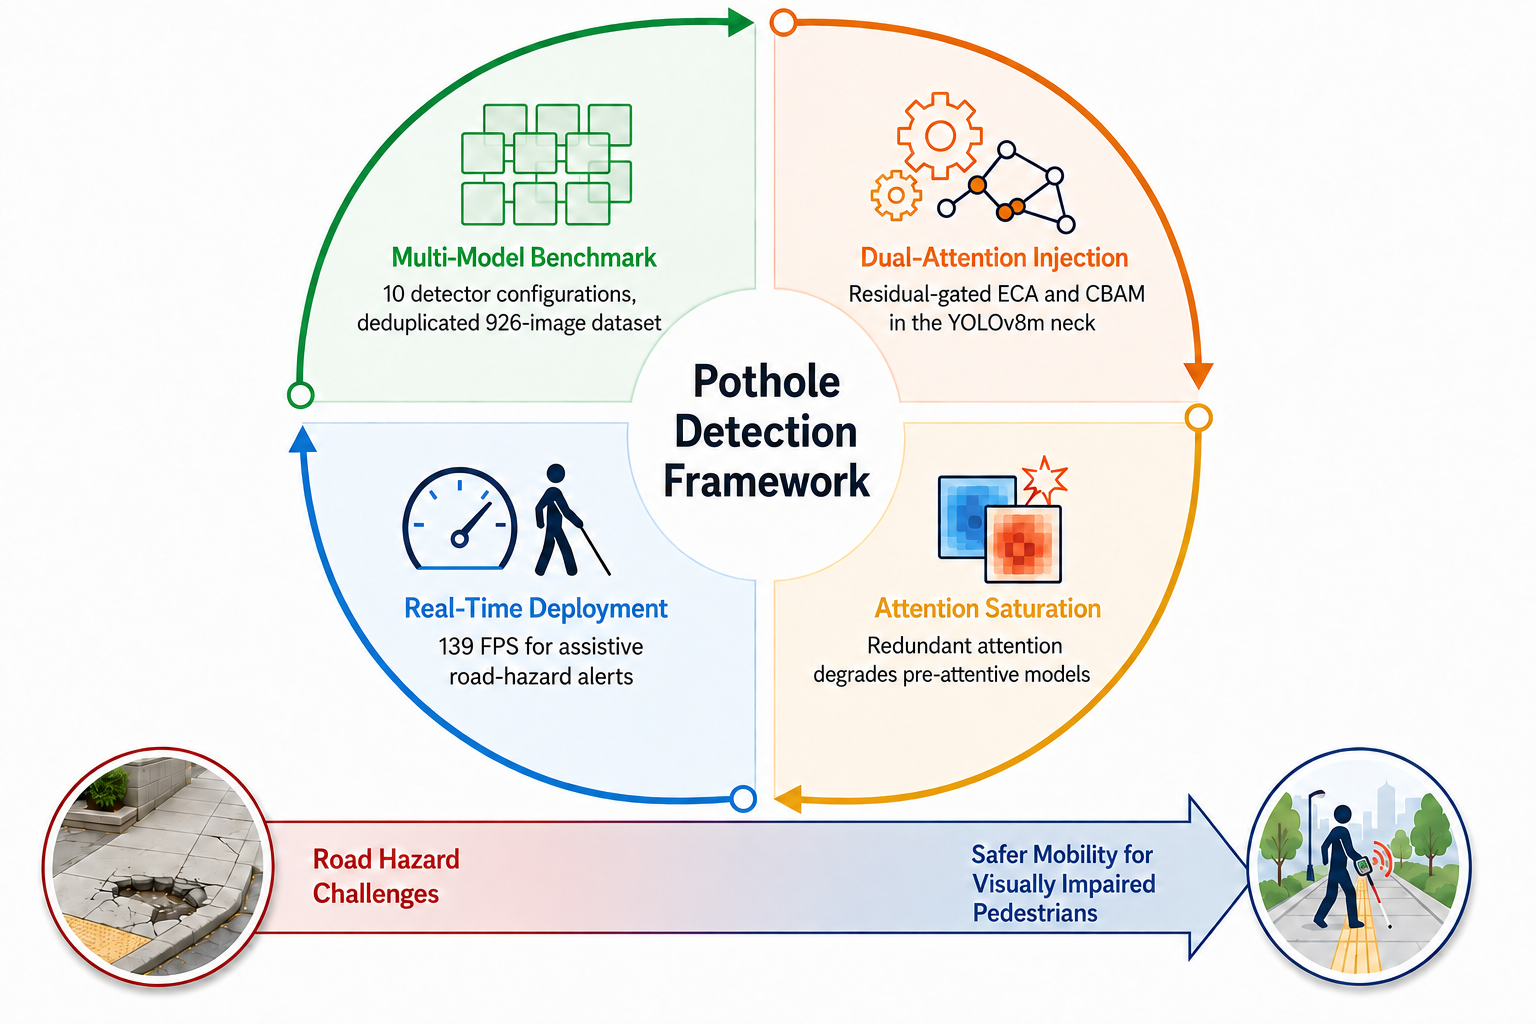
\includegraphics[width=0.70\textwidth]{fig1_intro_framework.png}
   \caption[Overview of the proposed framework.]
           {\label{fig:intro_framework}Overview of the RGDA-YOLOv8m pothole
            detection framework: dataset consolidation and deduplication, the
            residual-gated dual-attention architecture, the cross-architecture
            benchmark, and the ablation and architecture-dependence analyses.}
\end{figure}

\section{Contributions}
\label{sec:contributions}

The contributions of this dissertation are as follows. Throughout, detection
accuracy is reported as mean average precision at an intersection-over-union
threshold of 0.5, written mAP@0.5, and throughput is reported in frames per
second (FPS).

\begin{itemize}
   \item \textbf{A deduplicated multi-source pothole dataset and the procedure
      that produced it.} Three public Kaggle repositories were consolidated and
      then deduplicated by normalized-pixel nearest-neighbor matching, which
      removed 1,078 of 2,004 images, more than half the corpus, because
      the repositories redistribute overlapping data. Byte-level hashing was
      tried first and failed, for reasons documented in
      Chapter~\ref{ch:dataset}. The resulting corpus contains 926 images and
      2,354 annotations.

   \item \textbf{A controlled ten-configuration benchmark.} RGDA-YOLOv8m and
      nine comparators (YOLOv8m, YOLOv10m, YOLOv11m, Faster R-CNN,
      SSD-VGG16, RT-DETR, a YOLOv8m and Faster R-CNN ensemble combined by
      Weighted Box Fusion, YOLOv8m+CBAM and YOLOv8m+CoordAttn) are evaluated
      on the same 186-image validation partition under one average-precision
      definition and one throughput-measurement procedure.

   \item \textbf{The RGDA-YOLOv8m architecture.} Sequential ECA and CBAM
      refinement is applied at three YOLOv8m neck stages and combined with the
      unrefined features through a learnable scalar gate initialised to zero,
      so the network at initialisation is exactly the pretrained detector.
      Across three seeds the model attains an mAP@0.5 of $0.8141 \pm 0.0142$
      and an F1 of $0.7708 \pm 0.0121$, improvements of 0.82 and 1.07
      percentage points over the identically trained baseline, for 64,824
      additional parameters (0.25\%) and 139.9 FPS.

   \item \textbf{A factorial ablation of the two attention pathways.} The
      no-attention, ECA-only, CBAM-only and combined conditions are compared
      under an identical training schedule across three seeds. Neither single
      module improves on the baseline. Only the combination does.

   \item \textbf{The attention-saturation result.} Attaching the identical
      block to YOLOv11m reduces both mAP@0.5 and F1 at every seed. The
      comparison is against a single-run baseline and so is weaker than the
      three-seed YOLOv8m ablation, but it is the result with the broadest
      implication: the benefit of an added attention module may be a property
      of the pairing rather than of the module.

   \item \textbf{An account of protocol sensitivity.} Three methodological
      choices (deduplication, the average-precision definition, and the
      throughput-measurement method) are each shown to move the reported
      numbers by more than the architectural effect under investigation.
\end{itemize}

\section{Thesis Structure}
\label{sec:thesis_structure}

Chapter~\ref{ch:related} reviews classical, CNN-based, YOLO-family,
attention-enhanced and ensemble approaches to pothole and road-damage
detection, together with the datasets and evaluation practices of the field.
Chapter~\ref{ch:architectures} describes the detector architectures used in the
benchmark and the software framework within which they were extended.
Chapter~\ref{ch:dataset} documents the construction, deduplication and
statistical properties of the dataset. Chapter~\ref{ch:method} presents the
design of the residual-gated dual-attention block, its integration by forward
hooks, and the two-phase training protocol.
Chapter~\ref{ch:metrics} specifies the evaluation metrics and the measurement
procedures used to obtain them. Chapter~\ref{ch:results} reports and discusses
the benchmark, the multi-seed evaluation, the ablation, the
architecture-dependence experiment and the speed--accuracy trade-off.
Chapter~\ref{ch:conclusion} draws the conclusions, states the
limitations and sets out directions for further work.


%%%%%%%%%%%%%%%%%%%%%%%
% CHAPTER 2 -- Related Work
%%%%%%%%%%%%%%%%%%%%%%%

\chapter{Related Work}
\label{ch:related}

This chapter reviews the literature that positions the work reported here:
classical image processing and non-visual sensing; the transition to
convolutional detection; YOLO-family architectures adapted for road defects;
attention mechanisms in detection architectures; transformer-based detection;
ensemble and fusion approaches; and the datasets and evaluation practices that
determine whether any of these results can be compared with one another. It
closes by stating the gaps that the work reported here addresses.

\section{Classical and Sensor-Based Pothole Detection}
\label{sec:classical}

The earliest vision-based detectors were built from explicit rules about what a
pothole looks like: Koch and Brilakis \parencite{koch2011pothole} segment a
pavement image by histogram-shape-based thresholding, approximate each
candidate's shape by morphological thinning and elliptic regression, and accept
or reject it by comparing interior and surrounding texture, while related work
applied edge detectors and the Hough transform to video
\parencite{nienaber2015detecting}. Such methods need no training data and fail
legibly, but their assumptions are fixed at design time while the confounders
listed in Section~\ref{sec:what_makes_hard} are not, so they grow brittle in
proportion to the special cases they accumulate. Vision is not the only
modality: Pothole Patrol \parencite{eriksson2008pothole} inferred anomalies from
the vertical acceleration of taxi suspensions, turning a fleet into a survey
instrument at almost no marginal cost, but a vibration sensor reports only
defects the vehicle drives over and only after contact. Three-dimensional
methods instead measure the surface geometrically, and Fan et
al.~\parencite{fan2022rethinking} show that fitting a reference plane to a
reconstruction isolates depressions in a way largely immune to appearance
confounds. Ma et al.~\parencite{ma2022computer} organise the field along this
axis and note that the sensing hardware 3-D reconstruction requires is what has
kept it out of consumer-scale deployment.


\section{Convolutional Detection for Road Damage}
\label{sec:cnn_rdd}

Convolutional methods entered this domain as patch classification, when Zhang et
al.~\parencite{zhang2016road} showed a learned representation outperforming
handcrafted descriptors on the same data. Yang et
al.~\parencite{yang2020automated} extended this to pixel-level segmentation and
Li et al.~\parencite{li2023pavement} added uncertainty estimation, segmentation
suiting quantification of a defect's area and detection suiting warning or
triage, as here. Detection proper was driven by the road-damage challenges:
Maeda et al.~\parencite{maeda2018road} trained an SSD-based detector on
municipal smartphone imagery, showing a single-stage detector on commodity
hardware could produce usable survey data, and Wang et
al.~\parencite{wang2020road} found cross-city generalisation markedly worse than
within-city, an early sign of location-specific appearance bias. The two-stage
lineage from R-CNN \parencite{girshick2014rcnn} to Faster R-CNN
\parencite{ren2015faster} localises well but at substantial cost, appearing here
mainly as an ensemble component. Al-Shaghouri et
al.~\parencite{alshaghouri2021realtime} give the most careful pothole-specific
comparison, evaluating SSD, YOLOv3 and YOLOv4 on 1,087 images under matched
conditions, YOLOv4 reaching 85.39\% mAP at roughly 20 FPS with reliable
detection to one hundred metres, a range that determines how much warning time
the user gets.


\section{YOLO-Family Architectures for Road Defect Detection}
\label{sec:yolo_family}

The YOLO family reformulated detection as a single regression from image to
boxes and class scores \parencite{redmon2016yolo}, which is what makes it fast
enough for video. YOLOv8 \parencite{ultralytics2023yolov8} pairs C2f blocks,
built on the residual-learning principle of \textcite{he2016resnet}, with a
PAN-FPN neck and an anchor-free decoupled head, addressing the
foreground--background imbalance of dense prediction by task-aligned assignment
rather than focal loss \parencite{lin2017focal}. YOLOv10
\parencite{wang2024yolov10} added dual assignments so that non-maximum
suppression can be dropped at inference; and YOLO11
\parencite{ultralytics2024yolov11} replaced C2f with C3k2 blocks and, critically
here, inserted a C2PSA partial-self-attention module after the backbone's
spatial pyramid pooling stage, each version embedding more attention-like
machinery in the base architecture. Much later work adapts them for
constrained hardware or multi-scale fusion
\parencite{li2024bseyolo,he2024lmferdd,pei2024yolordd}. Two findings bear
directly on this study: LRS-YOLO gains 7.2 percentage points of mAP@50 on
RDD2022 but only 2.8 on UAV-PDD2023 \parencite{chen2024lrsyolo}, the
dataset-side analogue of the architecture-side dependence examined here, and
Pham et al.~\parencite{pham2024optimizing} report that newer YOLO versions did
not uniformly outperform older ones once inference time was accounted for, as
Chapter~\ref{ch:results} also finds. For scale, Abdelwahed et
al.~\parencite{abdelwahed2025advancements} benchmark YOLOv10m, v11m and v12m at
0.511, 0.515 and 0.525 mAP@0.5:0.95 and 223, 213 and 206 FPS.


\section{Attention Mechanisms in Detection Architectures}
\label{sec:attention_related}

Channel attention began with Squeeze-and-Excitation \parencite{hu2018squeeze},
which pools each channel to a scalar and rescales it but forces every channel
interaction through a bottleneck. Efficient Channel Attention
\parencite{wang2020eca} replaced that bottleneck with a small one-dimensional
convolution, Coordinate Attention \parencite{hou2021coordinate} factorised the
pooling to retain positional structure, the Convolutional Block Attention Module
\parencite{woo2018cbam} added a spatial gate after a channel gate, BAM
\parencite{park2018bam} arranged the two in parallel, and non-local networks
\parencite{wang2018nonlocal} generalised spatial attention to explicit
long-range interaction. ECA and CBAM are specified in full in
Chapter~\ref{ch:method}. Results in road-damage papers are almost uniformly
positive \parencite{pei2024yolordd,chen2024lrsyolo,pham2024optimizing}, two
being directly relevant: YOLO9tr \parencite{youwai2024yolo9tr} found a
single-attention-step variant underperforming its full configuration, and Zhang
et al.~\parencite{zhang2025automatic} add attention beneficially to a YOLOv11
host, raising mAP@0.50 from 88.2\% to 91.2\%, the opposite of what
Chapter~\ref{ch:results} observes and a tension taken up in
Section~\ref{sec:disc_saturation}. Interpretation is complicated by attention
rarely being introduced alone
\parencite{chen2024lrsyolo,pei2024yolordd,zhang2025automatic,lu2025fmsyolo} and
by single-run ablations that confound it with run-to-run variation.
Underneath lies an unexamined assumption: attaching a module to one host
estimates an effect size only if that effect is host-independent. No study
located here tests that by holding the block and protocol fixed and varying only
the host.


\section{Transformer-Based Detection}
\label{sec:transformers_related}

DETR \parencite{carion2020detr} reformulated detection as direct set prediction
over CNN features with a bipartite matching loss, removing both anchors and
non-maximum suppression, and the self-attention it inherits from the transformer
architecture \parencite{vaswani2017attention} gives every feature position
access to every other, which is qualitatively different from the local
reweighting performed by modules such as CBAM. Its practical weaknesses were
slow convergence and poor small-object performance. RT-DETR
\parencite{zhao2024rtdetr} addressed the speed problem with a hybrid encoder
decoupling intra-scale interaction from cross-scale fusion, achieving throughput
competitive with YOLO detectors while retaining NMS-free set prediction, and is
this dissertation's representative of that paradigm. As Chapter~\ref{ch:results}
shows, its confidence calibration differs from that of NMS-based detectors in a
way that has direct consequences for how detectors should be compared. The Swin
Transformer \parencite{liu2021swin} made transformer backbones practical for
dense prediction and appears in road-damage systems such as the ensemble of Ding
et al.~\parencite{ding2022ensemble}. The relevance here is conceptual, since
Swin, C2PSA and the partial attention block of YOLO9tr all place self-attention
inside the feature extractor, precisely the condition under which
Chapter~\ref{ch:results} suggests further external attention becomes
counterproductive.


\section{Ensemble and Fusion Approaches}
\label{sec:ensembles_related}

Combining detectors requires deciding what to do with overlapping boxes:
non-maximum suppression discards every box overlapping a higher-scoring one
beyond a threshold and Soft-NMS \parencite{bodla2017soft} decays their scores
instead, but both are suppression rules, so the surviving box is one of the
inputs and the information in the discarded boxes is lost, whereas Weighted Box
Fusion \parencite{solovyev2021weighted} clusters overlapping detections and
computes a fused box whose coordinates are a confidence-weighted average of the
cluster members, exploiting the partly independent localisation errors of
independent detectors at the cost of running every member model. Ding et
al.~\parencite{ding2022ensemble} built an ensemble of one-stage, two-stage and
Swin-Transformer-based detectors for the CRDDC2022 challenge and report a mean
F1 of 0.7699 across three country subsets, a representative result in that
ensembling reliably improves accuracy on road-damage benchmarks and reliably
destroys real-time throughput. This dissertation includes a YOLOv8m and Faster
R-CNN ensemble combined by Weighted Box Fusion specifically to quantify that
exchange on the same data as the single-model configurations.


\section{Datasets, Evaluation and Comparability}
\label{sec:datasets_related}

Road-damage research is organised around a few public corpora: RDD2022
\parencite{arya2022rdd2022} underpins the CRDDC challenges. UAV-PDD2023 supplies
aerial imagery on which Pan et al.~\parencite{pan2025realtime} report an mAP@0.5
of 0.542, a reminder that reported accuracy is dominated by task difficulty
rather than architecture quality. Pothole-specific work relies on Kaggle
repositories \parencite{chitholian_dataset,andrewmvd_dataset,ashishkumarak_dataset}
that are convenient, small and, as Chapter~\ref{ch:dataset} shows, substantially
overlapping; and robustness-oriented corpora are rare, Frnda et
al.~\parencite{frnda2024analysis} being an exception in spanning clear, rainy,
night, evening and sunset conditions and finding accuracy degrading sharply
under adverse illumination. The overlap matters, because a re-encoded copy of an
image appearing in both partitions inflates every metric invisibly, and very few
studies report a deduplication step. Nor is average precision a single quantity:
the VOC 2007 rule averages interpolated precision at eleven recall levels while
COCO integrates over 101 \parencite{everingham2010pascal,lin2014microsoft},
giving different numbers from identical predictions, and frames per second is
worse still. Compounding this, most studies report one run without any estimate
of its variance, so no later reader can tell whether two results are consistent.
The three-seed protocol adopted here is a minimal response.


\section{Synthesis and Research Gaps}
\label{sec:related_synthesis}

Table~\ref{tab:related} summarises the studies most directly relevant to this
dissertation and states what each contributes to it.

\begingroup
\small
\setlength{\tabcolsep}{4pt}
\begin{xltabular}{\textwidth}{@{}>{\raggedright\arraybackslash}p{3.4cm}
                                 >{\raggedright\arraybackslash}p{3.6cm}
                                 >{\raggedright\arraybackslash}X@{}}
\caption[Studies most relevant to this dissertation.]
        {Studies most directly relevant to this dissertation and the role each
         plays in it.}\label{tab:related}\\
\toprule
\textbf{Study} & \textbf{Approach} & \textbf{Relevance to this work} \\
\midrule
\endfirsthead

\multicolumn{3}{@{}l}{\footnotesize\emph{Table~\thetable\ (continued from previous page)}}\\
\toprule
\textbf{Study} & \textbf{Approach} & \textbf{Relevance to this work} \\
\midrule
\endhead

\midrule
\multicolumn{3}{r@{}}{\footnotesize\emph{Continued on next page}}\\
\endfoot

\bottomrule
\endlastfoot

\textcite{koch2011pothole}
   & Histogram thresholding, morphology, texture comparison
   & Establishes the appearance assumptions that learned detectors remove \\
\addlinespace[3pt]
\textcite{eriksson2008pothole}
   & Accelerometer and GPS sensing
   & Contrasting modality; motivates forward-looking vision \\
\addlinespace[3pt]
\textcite{ma2022computer}
   & Review of road imaging and pothole detection
   & Organises the sensing and algorithmic design space \\
\addlinespace[3pt]
\textcite{maeda2018road}
   & SSD on municipal smartphone imagery
   & Demonstrates single-stage feasibility at survey scale \\
\addlinespace[3pt]
\textcite{alshaghouri2021realtime}
   & SSD, YOLOv3, YOLOv4 compared on 1,087 pothole images
   & Matched-protocol comparison; detection range matters for warning \\
\addlinespace[3pt]
\textcite{ren2015faster}
   & Faster R-CNN with region proposal network
   & Supplies the two-stage comparator and the ensemble member \\
\addlinespace[3pt]
\textcite{zhao2024rtdetr}
   & Real-time DETR with hybrid encoder
   & Supplies the set-prediction comparator; motivates dual operating points \\
\addlinespace[3pt]
\textcite{wang2020eca}
   & Efficient Channel Attention
   & Channel-recalibration component of the proposed block \\
\addlinespace[3pt]
\textcite{woo2018cbam}
   & Sequential channel and spatial attention
   & Channel--spatial component of the proposed block \\
\addlinespace[3pt]
\textcite{hou2021coordinate}
   & Direction-aware channel attention
   & Alternative attention comparator in the benchmark \\
\addlinespace[3pt]
\textcite{pei2024yolordd}
   & YOLOv8 with DSC-C2f and coordinate attention
   & Representative positive attention result on a YOLOv8 host \\
\addlinespace[3pt]
\textcite{chen2024lrsyolo}
   & YOLOv8n with RFAConv, SPPFCSPPC and LKCA
   & Shows the same modification giving very different gains per dataset \\
\addlinespace[3pt]
\textcite{zhang2025automatic}
   & Improved YOLOv11 with fusion attention
   & Reports attention gains on a YOLOv11 host; contrasted in Chapter~\ref{ch:results} \\
\addlinespace[3pt]
\textcite{youwai2024yolo9tr}
   & YOLOv9 with a partial attention block
   & Reports that the number of attention stages matters independently \\
\addlinespace[3pt]
\textcite{ding2022ensemble}
   & One-stage and two-stage ensemble for CRDDC2022
   & Establishes the ensemble accuracy--throughput exchange \\
\addlinespace[3pt]
\textcite{solovyev2021weighted}
   & Weighted Box Fusion
   & Fusion rule used to build the ensemble comparator \\
\addlinespace[3pt]
\textcite{frnda2024analysis}
   & YOLOv7 and Faster R-CNN under five weather conditions
   & Identifies the robustness limitation of fair-weather corpora \\
\addlinespace[3pt]
\textcite{paramarthalingam2024pothole}
   & YOLOv5 for assistive pothole detection
   & Closest application match; external accuracy reference point \\
\end{xltabular}
\endgroup

Three gaps follow from this review, and they are what the objectives of
Section~\ref{sec:gap_objectives} address. First, no located study places
one-stage, two-stage, transformer-based, attention-enhanced and ensemble
detectors on a single deduplicated pothole dataset under one fully specified
protocol. Second, no located study isolates the individual and joint
contributions of a channel and a spatial attention pathway inserted at the same
locations under an identical schedule. Third, and most importantly,
no located study holds the attention block and training protocol fixed and
varies only the host architecture in order to test whether the benefit of
attention is a property of the module or of the pairing.


%%%%%%%%%%%%%%%%%%%%%%%
% CHAPTER 3 -- Detector Architectures and Experimental Framework
%%%%%%%%%%%%%%%%%%%%%%%

\chapter{Detector Architectures and Experimental Framework}
\label{ch:architectures}

This chapter describes the detection architectures evaluated in this
dissertation and the software framework within which they were trained,
extended and measured. Its purpose is to make the later chapters legible: the
design of the proposed attention block in Chapter~\ref{ch:method} depends on
specific structural properties of the YOLOv8m neck, and the
architecture-dependence result in Chapter~\ref{ch:results} depends on a
specific structural difference between YOLOv8m and YOLOv11m. Both are set out
here.

\section{Anatomy of a Modern Detector}
\label{sec:detector_anatomy}

\subsection{Backbone, Neck and Head}

Contemporary convolutional detectors share a three-part decomposition. The
\emph{backbone} is a convolutional feature extractor that consumes the input
image and produces a pyramid of feature maps at progressively lower spatial
resolution and higher channel dimension. The stages of that pyramid are
conventionally labelled P1 to P5, where P$n$ has been downsampled by a factor
of $2^{n}$. For a $640 \times 640$ input the P3, P4 and P5 stages have spatial
resolutions of $80 \times 80$, $40 \times 40$ and $20 \times 20$ respectively.
Shallow stages retain spatial detail but encode weak semantics. Deep stages
encode strong semantics but have lost the resolution needed to localise small
objects.

The \emph{neck} exists to resolve that tension. A Feature Pyramid Network
\parencite{lin2017fpn} propagates semantic information downward from deep
stages to shallow ones through a top-down path with lateral connections, so
that the high-resolution features used to detect small objects are
semantically informed. PANet \parencite{liu2018panet} adds a second,
bottom-up path so that the precise localisation signal available in shallow
layers also propagates upward. The combination, referred to as PAN-FPN, is the
neck design used by YOLOv8 and its immediate successors.

The \emph{head} converts each neck output into predictions. A detection is
produced at each spatial position of each pyramid level, so the three levels
naturally specialise to small, medium and large objects.

\subsection{Anchor-Free Prediction and Label Assignment}

Older detectors predicted offsets relative to a fixed set of anchor boxes whose
sizes and aspect ratios had to be chosen in advance, often by clustering the
training annotations. Anchor-free detectors such as FCOS
\parencite{tian2019fcos} instead regress the distances from each position to
the four sides of the box directly, which removes a set of dataset-specific
hyperparameters. YOLOv8 is anchor-free and uses a distribution-focal
formulation in which each box side is predicted as a discrete distribution over
candidate offsets rather than as a single scalar.

Label assignment, deciding which predicted positions are responsible for
which ground-truth boxes, is handled by a task-aligned assigner that scores
candidate positions by a combination of classification confidence and
localisation quality, rather than by the fixed geometric rules used in earlier
detectors. This matters for pothole detection because potholes have irregular
outlines that fill their bounding boxes poorly, so a purely geometric
assignment rule tends to select positions that lie on the road surface rather
than on the defect.

\subsection{Receptive Field and Small-Object Detection}

The reason multi-scale fusion is not optional for this task can be stated in
terms of receptive fields. A unit in the P5 stage of a YOLOv8 backbone responds
to a region of the input image spanning a large fraction of the frame, which is
what allows it to encode context, that this dark region sits in a road rather
than in foliage. A unit in P3 responds to a much smaller region and can
therefore resolve a defect only tens of pixels across, but has correspondingly
little context with which to distinguish it from a shadow.

Neither stage alone is adequate for potholes, because the same physical defect
appears at both scales depending on its distance from the camera. A pothole ten
metres ahead is a P5-scale object. The same pothole at sixty metres is a
P3-scale object, and it is the distant one whose detection provides useful
warning time. The corpus described in Chapter~\ref{ch:dataset} contains
instances across this entire range within single images, since a road scene
recedes towards a vanishing point and defects at several distances are
simultaneously visible.

The consequence for this dissertation's design is direct. If the detector's
difficulty is concentrated in reconciling scales, then the fusion stage is
where a content-dependent reweighting has the most to work with: it is the
only place in the network where features carrying fine spatial detail and
features carrying scene context are present in the same tensor. This is the
architectural argument for the injection points chosen in
Chapter~\ref{ch:method}, complementing the empirical argument from the dataset
properties given in Section~\ref{sec:dataset_stats}.

\subsection{Model Scaling and the Choice of the Medium Variant}

Ultralytics architectures are published in five sizes (n, s, m, l and x)
generated from one topology by two multipliers, one scaling channel width and
one scaling block repetition, so the variants differ only in width and depth.
The medium variant was used for every YOLO configuration in this dissertation.
The nano and small variants are the natural choice for embedded deployment and
dominate the lightweight-modification literature of Chapter~\ref{ch:related},
but they leave little headroom, so a 0.25 percent parameter addition sits closer
to the noise floor of what the architecture can express. The large and
extra-large variants would reduce throughput below the real-time threshold that
motivates the work. At approximately 25.9 million parameters and over 150 FPS on
the target hardware, the medium variant is the smallest configuration for which
an 8.1 percent throughput cost is clearly affordable and the largest for which
real-time operation is uncontroversial. Holding the scale fixed throughout is
also a control: comparing an attention-augmented small model against an
unaugmented medium one would confound the mechanism with capacity.

\subsection{The Role of Feature Recalibration}

Neither the backbone nor the neck contains any mechanism that explicitly
decides which channels or which spatial locations of a fused feature map are
informative. Convolution is content-agnostic in the sense that its weights are
fixed once training is complete and do not depend on the particular input.
Attention modules supply exactly this input-dependent reweighting, and the
neck is the natural place to apply it: it is where multi-scale information has
been combined but before predictions are formed, so a recalibration applied
there influences every subsequent prediction at that scale. This observation
motivates the injection points chosen in Chapter~\ref{ch:method}.

\section{YOLOv8m: The Host Architecture}
\label{sec:yolov8m}

\subsection{C2f Feature Extraction}

The YOLOv8 backbone is built from C2f blocks \parencite{ultralytics2023yolov8}.
A C2f block splits its input along the channel dimension, routes one part
through a sequence of bottleneck units, and concatenates the outputs of every
bottleneck with the untransformed part before a final projection. Compared with
the C3 block it replaces, C2f exposes more gradient paths for the same
parameter budget, which improves optimisation without increasing inference
cost proportionally. The backbone terminates in a spatial pyramid pooling --
fast (SPPF) module that applies successive max-pooling operations with a shared
kernel and concatenates the results, giving the deepest stage a large effective
receptive field at low cost.

\subsection{Inside the C2f Block}

Because the injection points of Chapter~\ref{ch:method} are C2f block outputs,
the block's internal structure determines what those outputs contain. A C2f
block first applies a $1 \times 1$ convolution that expands the input to twice
a working width, then splits the result into two halves along the channel
dimension. One half is passed through unchanged. The other is fed through a
chain of $n$ bottleneck units, each consisting of two $3 \times 3$
convolutions with an optional identity shortcut, and the output of \emph{every}
unit in the chain is retained. All retained tensors, the untouched half and
the $n$ intermediate outputs, are concatenated and projected back to the
target width by a final $1 \times 1$ convolution.

Two properties follow. First, the block's output is a concatenation of
representations computed at different effective depths, so its channels are
heterogeneous by construction: some describe features that have passed through
one bottleneck, others through several, and one group through none at all.
Channel attention applied to such a tensor is therefore not merely selecting
among redundant filters but selecting among representations of genuinely
different character, which is a plausible reason for it to be useful here.
Second, retaining every intermediate output creates multiple short gradient
paths from the block output back to its input, which is the optimisation
benefit C2f was introduced to obtain.

The backbone closes with an SPPF module, which applies the same $5 \times 5$
max-pooling operation three times in succession and concatenates the input with
all three pooled results. Chaining a single kernel reproduces the effective
receptive fields of larger kernels at a fraction of the cost, and the
concatenation gives the deepest stage a representation that mixes several
context scales. In YOLO11 this is exactly the point at which the C2PSA
self-attention module is inserted, which is why the difference between the two
hosts is a difference in what the \emph{deepest} features have already
undergone.

\subsection{The PAN-FPN Neck}

The YOLOv8 neck implements the PAN-FPN pattern described above. The top-down
path upsamples P5, concatenates it with P4 and processes the result through a
C2f block. The output is upsampled again, concatenated with P3 and processed
through a further C2f block, yielding the highest-resolution neck output. The
bottom-up path then downsamples that output, concatenates it with the
intermediate top-down result and processes it, and repeats once more against
P5. The three C2f blocks that terminate these fusion paths are the outputs
delivered to the head.

For the medium-sized YOLOv8m configuration used throughout this dissertation,
these three blocks emit feature maps with 192, 384 and 576 channels
respectively. These are the three tensors that the attention block of
Chapter~\ref{ch:method} intercepts, and the channel dimensions determine the
parameter cost of the injected modules.

\subsection{The Decoupled Head}

YOLOv8 uses a decoupled head: classification and box regression are computed by
separate convolutional branches rather than from a shared output tensor. The
two tasks require different features (classification benefits from
translation invariance, localisation from translation equivariance), and
separating them measurably improves both. There is no objectness branch.
Classification confidence serves directly as the detection score.

\subsection{Rationale for YOLOv8m as the Host}

Three considerations led to YOLOv8m being selected as the host architecture for
the proposed modification. First, it contains no attention mechanism of its
own, which makes it a clean substrate: any effect observed can be attributed to
the injected modules rather than to an interaction with an existing one.
Second, the medium configuration at approximately 25.9 million parameters
occupies the region of the accuracy--throughput curve relevant to real-time
deployment on desktop-class hardware, so a throughput cost measured against it
is meaningful. Third, it is the most widely used baseline in the recent
road-damage literature reviewed in Chapter~\ref{ch:related}, which makes the
results interpretable against that literature.

\section{The Training Objective}
\label{sec:loss}

The loss function is specified here because it is common to every YOLO-family
configuration in this dissertation, including the proposed model, and because
the ablation of Chapter~\ref{ch:method} holds it fixed. YOLOv8 optimises a
weighted sum of three terms computed over the positions selected by the
task-aligned assigner:

\begin{equation}
   \mathcal{L} \;=\;
      \lambda_{\mathrm{cls}} \mathcal{L}_{\mathrm{cls}}
      \;+\; \lambda_{\mathrm{box}} \mathcal{L}_{\mathrm{box}}
      \;+\; \lambda_{\mathrm{dfl}} \mathcal{L}_{\mathrm{dfl}} .
   \label{eq:loss}
\end{equation}

The classification term $\mathcal{L}_{\mathrm{cls}}$ is binary cross-entropy
over class logits. With a single class it reduces to a
defect-versus-background decision at each selected position, which is
substantially easier than the multi-class discrimination required by the
road-damage benchmarks of Chapter~\ref{ch:related} and is one reason absolute
mAP values here are not comparable with those reported on RDD2022.

The localisation term $\mathcal{L}_{\mathrm{box}}$ is a complete-IoU loss,
which augments the plain IoU objective with penalties on the distance between
box centres and on aspect-ratio mismatch. This matters for potholes
specifically: an IoU-only objective provides no gradient when the predicted and
ground-truth boxes are disjoint, which is a common early-training condition for
small, low-contrast objects, whereas the centre-distance term remains
informative there.

The distribution-focal term $\mathcal{L}_{\mathrm{dfl}}$ supervises the
discretised box representation described in
Section~\ref{sec:detector_anatomy}. Because each box side is predicted as a
distribution over candidate offsets rather than as a scalar, the loss
encourages probability mass to concentrate on the two bins adjacent to the true
offset. The practical effect is that the model can express uncertainty about a
boundary rather than being forced to commit to a point estimate, which is
appropriate for potholes, whose edges are genuinely ambiguous. Several of the
road-damage detectors reviewed in Chapter~\ref{ch:related} modify this term,
substituting shape-aware IoU variants \parencite{lu2025fmsyolo,gao2025glbdetr}.
No such modification is made here, precisely so that the effect attributed to
the attention block is not confounded with a change of objective.

The loss weights, the assigner and the augmentation policy were left at their
Ultralytics defaults for every configuration. This is a deliberate constraint
rather than an omission: tuning them per configuration would improve absolute
results while destroying the controlled comparison that the ablation and the
architecture-dependence experiment depend on.

\section{Contemporary YOLO Variants}
\label{sec:yolo_variants}

YOLOv10 \parencite{wang2024yolov10} is included as the throughput-oriented
member of the family. It trains with consistent dual label assignments, a
one-to-many branch supplying rich supervision alongside a one-to-one branch
producing a single prediction per object, so that non-maximum suppression can
be removed at inference without the accuracy loss a naive one-to-one assignment
would incur.

YOLO11 \parencite{ultralytics2024yolov11} revises feature extraction, replacing
C2f with C3k2 blocks that use smaller kernels in their bottleneck units, and
introduces a C2PSA module positioned immediately after the SPPF stage at the
end of the backbone. C2PSA applies \emph{partial self-attention}: the input is
split along channels, one part is processed through a self-attention block with
an accompanying feed-forward network, and the result is concatenated with the
untouched remainder. Self-attention here operates over spatial positions, so
each position of the deepest feature map is reweighted according to its
relationship with every other position.

The architectural consequence is central to this dissertation. In YOLOv8m, the
features arriving at the neck have never been reweighted by any
content-dependent mechanism. In YOLOv11m, they have: the deepest backbone
stage has already undergone a round of spatial self-attention before the neck
begins fusing scales. If the value of an added attention module lies in
performing a recalibration the host has left undone, then the same module
attached to these two hosts should not behave the same way. This is precisely
the comparison performed in Section~\ref{sec:results_saturation}.

\section{Non-YOLO Comparators}
\label{sec:non_yolo}

\subsection{Faster R-CNN}

Faster R-CNN \parencite{ren2015faster} is the two-stage representative. A
region proposal network slides over the backbone feature map and emits
class-agnostic object proposals with objectness scores. A second stage pools
features from each proposal to a fixed size and classifies and refines it. The
configuration used here is the ResNet-50-FPN-v2 variant with COCO-pretrained
weights. Two-stage detection generally localises well because the second stage
sees features aligned to a hypothesised object rather than to a fixed grid, at
the cost of running that stage once per proposal.

\subsection{SSD-VGG16}

SSD \parencite{liu2016ssd} predicts boxes directly from multiple feature-map
scales using fixed anchor boxes, with no proposal stage and no feature-pyramid
fusion. It is included as a high-throughput, architecturally simple lower
bound. It is used at its native $300 \times 300$ input resolution with a VGG16
backbone, which is a genuine disadvantage relative to the $640 \times 640$
inputs of the other configurations and is accounted for when its results are
interpreted.

\subsection{RT-DETR}

RT-DETR \parencite{zhao2024rtdetr} is the set-prediction representative,
evaluated from the \texttt{rtdetr-l.pt} COCO-pretrained checkpoint. Its
efficient hybrid encoder separates intra-scale feature interaction, performed
by self-attention on the deepest level only, from cross-scale fusion, performed
by convolution, which is what makes transformer-based detection fast enough for
this comparison. Because it produces a fixed-size set of predictions without
non-maximum suppression, its confidence scores are distributed differently from
those of NMS-based detectors, a property that turns out to matter a great
deal in Chapter~\ref{ch:results}.

\subsection{The Weighted Box Fusion Ensemble}

The ensemble comparator combines the predictions of the fine-tuned YOLOv8m and
Faster R-CNN models using Weighted Box Fusion
\parencite{solovyev2021weighted}. Detections from both models are pooled,
clustered by overlap, and each cluster is replaced by a single box whose
coordinates are the confidence-weighted mean of the cluster members and whose
score reflects both the members' scores and the number of models contributing.
The relative model weights were swept over $[0.3, 0.7]$. No additional training
is involved: the ensemble reuses predictions already produced by its members,
so its accuracy is obtained entirely at the cost of running both models.

Table~\ref{tab:baselines} summarises all ten configurations evaluated in this
dissertation, the six described in this section together with the YOLO-family
models of Sections~\ref{sec:yolov8m} and~\ref{sec:yolo_variants} and the two
single-attention comparators.

\begin{table}[tbp]
\centering
\small
\setlength{\tabcolsep}{4pt}
\begin{tabularx}{\textwidth}{@{}>{\raggedright\arraybackslash}p{3.1cm}
                                >{\raggedright\arraybackslash}p{2.2cm} X@{}}
\toprule
\textbf{Configuration} & \textbf{Family} & \textbf{Description} \\
\midrule
YOLOv8m & One-stage & C2f backbone, PAN-FPN neck, anchor-free decoupled head;
   approximately 25.9M parameters, COCO-pretrained. Host architecture and
   principal baseline. \\
\addlinespace[8pt]
YOLOv10m & One-stage & Consistent dual assignments permitting NMS-free
   inference; throughput-oriented family member. \\
\addlinespace[8pt]
YOLOv11m & One-stage & C3k2 blocks with a C2PSA partial self-attention module
   after SPPF; the host used to test architecture dependence. \\
\addlinespace[8pt]
Faster R-CNN & Two-stage & ResNet-50-FPN-v2 with region proposal network and
   RoI feature pooling, COCO-pretrained. \\
\addlinespace[8pt]
SSD-VGG16 & One-stage & Multiscale anchor prediction on a VGG16 backbone at
   native $300 \times 300$ resolution. \\
\addlinespace[8pt]
RT-DETR & Set prediction & Convolutional backbone, efficient hybrid encoder,
   transformer decoder; \texttt{rtdetr-l.pt} checkpoint, NMS-free. \\
\addlinespace[8pt]
YOLO+FRCNN (WBF) & Ensemble & YOLOv8m and Faster R-CNN predictions fused by
   Weighted Box Fusion, model weights swept over $[0.3,0.7]$. \\
\addlinespace[8pt]
YOLOv8m+CBAM & Attention & CBAM at the same three neck blocks, same
   zero-initialised gate and two-phase schedule as the proposed model, without
   the preceding ECA stage. \\
\addlinespace[8pt]
YOLOv8m+CoordAttn & Attention & Coordinate Attention at the same three neck
   blocks under the same mechanism and schedule, substituting direction-aware
   pooling for CBAM's channel-then-spatial refinement. \\
\addlinespace[8pt]
\textbf{RGDA-YOLOv8m} & Attention & \textbf{Proposed.} Sequential ECA then CBAM
   at the same three neck blocks, combined with the unrefined features through
   a learnable scalar gate initialised to zero. \\
\bottomrule
\end{tabularx}
\caption[Configurations evaluated in the benchmark.]
        {\label{tab:baselines}The ten detector configurations evaluated. All
         were fine-tuned from COCO-pretrained initialisations on the same
         740-image training partition and evaluated on the same 186-image
         validation partition.}
\end{table}

\section{Software Framework and Extension Mechanism}
\label{sec:framework}

The YOLO-family and RT-DETR configurations were trained and evaluated through
the Ultralytics framework \parencite{ultralytics2023yolov8}, which builds on
PyTorch \parencite{paszke2019pytorch} and supplies the C2f blocks, PAN-FPN neck
and decoupled head described in Section~\ref{sec:yolov8m} together with the
training loop, validation-based checkpoint selection and the
\texttt{model.val()} evaluation routine. Faster R-CNN and SSD-VGG16 fall
outside it and were trained through torchvision with an explicit loop.

Modifying an Ultralytics model conventionally means one of two things, and both
were rejected here:

\begin{itemize}
   \item registering a new block type, which requires editing the framework
      source;
   \item writing a modified YAML topology, which shifts layer indices and so
      silently changes which layers the \texttt{freeze} parameter freezes.
\end{itemize}

Either route changes the model definition, so the modified and unmodified
detectors would no longer be guaranteed identical in every respect other than
the modification. For an experiment whose purpose is to attribute a
sub-percentage-point difference to one module, that is unacceptable.

The mechanism adopted instead is the PyTorch forward hook. Registered on a
chosen neck block, it receives that block's output tensor after the forward
method returns and may return a replacement, so the attention transformation is
applied without the block, the model definition, the layer indexing or the
framework source being altered at all, and the two runs differ in precisely one
respect. Because the modules are not registered as submodules, their parameters
are absent from the checkpoints Ultralytics writes and must be persisted
separately. A model distributed as weights alone reverts to an unmodified
detector, a limitation revisited in Section~\ref{sec:disc_limitations}.

\section{Experimental Pipeline and Hardware}
\label{sec:hardware}

Training the ten configurations across multiple seeds involves long-running GPU
jobs that can fail part-way through, so the pipeline writes a JSON record per
run on completion, holding the configuration, seed, every computed metric, the
confidence sweep and the measured throughput, alongside a per-group manifest
recording the environment, checkpoint paths and timestamps. An interrupted
experiment can therefore resume without repeating completed runs, and every
number in Chapter~\ref{ch:results} is traceable to the run that produced it.
All of those runs used a single NVIDIA GeForce RTX 3090 with 24\,GB of memory,
and every inference measurement reported in this dissertation uses FP32
precision at batch size one, the operating regime of a real-time streaming
application and a deliberately conservative choice, since batching and reduced
precision would raise every throughput figure without corresponding to the
deployment scenario the work targets. Because all configurations were measured
under identical conditions on identical hardware, the relative comparisons hold
even though the absolute figures are specific to this GPU.


%%%%%%%%%%%%%%%%%%%%%%%
% CHAPTER 4 -- Dataset Construction and Analysis
%%%%%%%%%%%%%%%%%%%%%%%

\chapter{Dataset Construction and Analysis}
\label{ch:dataset}

Every number reported in Chapter~\ref{ch:results} rests on the corpus described
here, and the single most consequential decision in this dissertation was made
at this stage rather than at the architectural one. This chapter documents the
three source repositories, the deduplication procedure that removed more than
half of their union, the unification of two incompatible annotation formats,
the partitioning scheme, and the resulting statistical properties of the data.
It closes with the threats to validity that the corpus imposes on everything
built on it.

\section{Source Repositories}
\label{sec:sources}

Three publicly available pothole datasets hosted on Kaggle were consolidated
into a single corpus. The first, \path{chitholian/annotated-potholes-dataset}
\parencite{chitholian_dataset}, contains 665 images with bounding-box
annotations in Pascal VOC XML format. The second,
\path{andrewmvd/pothole-detection} \parencite{andrewmvd_dataset}, also
contains 665 images with Pascal VOC XML annotations. The third,
\path{ashishkumarak/training-setzip} \parencite{ashishkumarak_dataset},
contains 674 images with annotations supplied as CSV bounding-box records.

The union therefore comprises 2,004 annotated images carrying 4,851
ground-truth boxes: 1,740 from each of the two VOC repositories and 1,371 from
the CSV repository. Multiple repositories were used deliberately. A
single small pothole dataset captures one photographer's equipment, one
geography and one set of lighting conditions, and a detector trained on it
learns those incidental regularities alongside the defect itself. Combining
independently assembled repositories broadens the appearance distribution, provided the repositories are in fact independent, which is the question the
next section addresses.

\section{Deduplication}
\label{sec:dedup}

\subsection{Why Byte-Level Hashing Failed}

The obvious way to find duplicate images is to hash the files and group the
collisions. This was attempted first, using MD5 over the raw file bytes, and it
proved unreliable in a specific and instructive way: the same procedure applied
to the same three repositories found 674 duplicates in one download session and
none in another.

The explanation is that Kaggle packages are not byte-stable. The same
photograph redistributed through two repositories is re-encoded (different
JPEG quantisation tables, different chroma subsampling, different metadata), so the files differ at the byte level while being visually identical. A hash
over the file contents is sensitive to exactly the differences that do not
matter and blind to the equivalence that does. Any procedure that depends on
byte equality is therefore not merely imperfect here but non-deterministic
across download sessions, which is disqualifying for a study that needs to be
reproducible.

\subsection{Normalized-Pixel Nearest-Neighbor Matching}

The procedure adopted instead operates on image content rather than file
content. Each image is converted to greyscale, resampled to a fixed
$64 \times 64$ grid using Lanczos interpolation, and flattened to a
4,096-element vector. Two images $I_a$ and $I_b$ are treated as duplicates when
the mean absolute difference between their normalized representations falls
below a threshold $\tau$ on a 0--255 intensity scale:

\begin{equation}
   d(I_a, I_b) \;=\; \frac{1}{4096}\sum_{k=1}^{4096}
      \bigl| \, \mathbf{v}_a[k] - \mathbf{v}_b[k] \, \bigr|
   \;<\; \tau,
   \qquad \tau = 1.0 .
   \label{eq:dedup}
\end{equation}

Greyscale conversion removes sensitivity to colour-space differences introduced
by re-encoding; downsampling to $64 \times 64$ removes sensitivity to
resolution differences and to the high-frequency artefacts that JPEG
compression introduces; and the mean absolute difference is a robust,
interpretable measure on a scale that can be reasoned about directly. Images
are processed in order, each compared against the set of already-retained
representations, and retained only if no retained image lies within $\tau$.
Every image appearing in more than one repository is therefore kept exactly
once, and its first-encountered copy is the one retained.

\subsection{Threshold Selection}

The threshold $\tau = 1.0$ was set by measuring $d$ on sampled pairs that had
been confirmed duplicate by inspection and on sampled unrelated pairs.
Confirmed duplicates measured between 0.10 and 0.50 mean absolute intensity
difference. Unrelated pairs measured far higher. The separation between the two
populations is therefore roughly an order of magnitude, and $\tau = 1.0$ sits
comfortably inside the gap rather than at a boundary where small changes in the
threshold would change the outcome. This insensitivity matters: a threshold
chosen at a point where the result varies rapidly would make the entire corpus, and hence every result in this dissertation, an artefact of an arbitrary
constant.

\subsection{Outcome}

The procedure removed 1,078 of the 2,004 images, and the distribution of those
removals is the substantive finding: the \texttt{andrewmvd} repository proved
almost entirely contained within \texttt{chitholian}, contributing only 9
unique images against 656 duplicates, a further 422 duplicates were removed
from \texttt{ashishkumarak} leaving 252, and \texttt{chitholian}, processed
first, retained all 665 by construction, as Table~\ref{tab:dataset} sets out.
Had the step been omitted, those 1,078 images, 54 percent of the corpus, would
each have had a near-identical twin in the data, the overwhelming majority of
which would straddle an 80:20 partition, so the detector would have been
evaluated substantially on images it had memorised and every metric would have
been inflated invisibly and by a margin far exceeding the sub-percentage-point
architectural effects this dissertation sets out to measure. The same lesson
was learned once more during the experimental work, when an early set of
baselines was inadvertently scored over the entire un-deduplicated corpus and
produced a Faster R-CNN recall of 0.9988 against an implied 4,851 ground-truth
boxes where the held-out partition contains 474. The pipeline now rejects any
baseline whose implied count does not match the partition being scored.
Chapter~\ref{ch:related} noted that few published pothole-detection studies
report a deduplication step, and Section~\ref{sec:disc_protocol} returns to the
general point these two episodes illustrate, that procedural errors in this
domain are larger than the architectural ones under study and announce
themselves as plausible numbers rather than as failures.

\begin{table}[tbp]
\centering
\small
\setlength{\tabcolsep}{4pt}
\begin{tabularx}{\textwidth}{@{}>{\RaggedRight\arraybackslash}X c rrr
   >{\RaggedRight\arraybackslash}X@{}}
\toprule
\textbf{Repository} & \textbf{Source} & \textbf{Images} & \textbf{Removed} &
\textbf{Retained} & \textbf{Annotation format} \\
\midrule
\texttt{chitholian}    & Kaggle & 665 & 0   & 665 & Pascal VOC XML \\
\texttt{andrewmvd}     & Kaggle & 665 & 656 & 9   & Pascal VOC XML \\
\texttt{ashishkumarak} & Kaggle & 674 & 422 & 252 & CSV bounding boxes \\
\midrule
\textbf{Total}         & ---    & \textbf{2{,}004} & \textbf{1{,}078} &
   \textbf{926} & Unified to YOLO format \\
\bottomrule
\end{tabularx}
\caption[Dataset composition before and after deduplication.]
        {\label{tab:dataset}Composition of the corpus before and after
         normalized-pixel nearest-neighbor deduplication. The union of the
         three repositories contains 4,851 annotated boxes. The deduplicated
         corpus contains 2,354.}
\end{table}

\section{Annotation Unification and Preprocessing}
\label{sec:preprocessing}

\subsection{Coordinate Conversion}

The three repositories supply annotations in two formats. Pascal VOC XML
records absolute pixel corner coordinates
$[x_{\min}, y_{\min}, x_{\max}, y_{\max}]$. The CSV repository records
bounding boxes as tabular rows. Both were converted to the YOLO convention of
normalized centre coordinates and normalized extents
$[c_x, c_y, w, h]$ \parencite{ultralytics2023yolov8}:

\begin{align}
   c_x &= \frac{x_{\min} + x_{\max}}{2W}, &
   c_y &= \frac{y_{\min} + y_{\max}}{2H}, \notag \\
   w   &= \frac{x_{\max} - x_{\min}}{W},  &
   h   &= \frac{y_{\max} - y_{\min}}{H},
   \label{eq:yolo_convert}
\end{align}

where $W$ and $H$ are the original image width and height. Normalization makes
the annotation independent of the image resolution, which is necessary because
the three repositories do not share one. The corpus contains a single object
class, \texttt{pothole}, so no class-taxonomy reconciliation was required, an advantage of pothole-specific data over the multi-class road-damage corpora
discussed in Chapter~\ref{ch:related}, where merging sources requires mapping
between incompatible damage taxonomies.

\subsection{Input Resolution and Augmentation}

All models except SSD-VGG16 were trained and evaluated at $640 \times 640$
pixels. SSD-VGG16 uses its native $300 \times 300$ resolution. Training
augmentation used the default Ultralytics pipeline: mosaic composition, which
tiles four training images into one and thereby increases the number of objects
and the diversity of contexts per training sample; random horizontal flipping;
HSV colour jitter, which is the augmentation most relevant to a task confounded
by illumination and surface colour; and random scaling. No augmentation was
applied at validation. The augmentation policy was held identical across all
configurations, so it cannot contribute to differences between them.

\section{Partitioning}
\label{sec:partitioning}

The deduplicated corpus was shuffled and divided into training and validation
partitions in an 80:20 ratio using a fixed random seed of 42, giving 740
training images and 186 validation images containing 474 annotated pothole
instances. This single canonical split is reused by every configuration and
every seed reported in this dissertation. The seed that controls the split is
deliberately independent of the seeds that control model initialisation and
data ordering: the three-seed protocol of Chapter~\ref{ch:metrics} varies
training stochasticity while holding the evaluation set exactly fixed, so that
run-to-run differences cannot be attributed to differences in what was being
measured.

No separate test partition was held out. With 926 images, splitting three ways
would leave a test set too small for the differences under study to be
resolvable at all. The consequence is that the validation partition serves both
for checkpoint selection in the YOLO-family models and for reporting, which
introduces an optimistic bias. That bias applies equally to every configuration
scored through \texttt{model.val()} and is stated as a limitation in
Section~\ref{sec:disc_limitations}.

\section{Characteristics of the Corpus}
\label{sec:dataset_stats}

The deduplicated corpus contains 926 images and 2,354 annotated pothole
instances, an average of 2.54 instances per image, with a maximum of 19
instances in a single image. This distribution is characteristic of the task:
most road scenes contain one or two clearly defined defects, while a minority
of images of severely deteriorated surfaces contain many small ones. The
long tail matters for evaluation, because a handful of dense images contribute
a disproportionate share of the total instance count and therefore a
disproportionate share of the recall denominator.

Figure~\ref{fig:dataset_samples} shows representative annotated images from the
three repositories, with ground-truth boxes drawn in green, blue and red
respectively for \texttt{chitholian}, \texttt{andrewmvd} and
\texttt{ashishkumarak}. The examples illustrate the appearance variation the
detector must accommodate: differences in pavement texture and colour, in
pothole morphology from shallow surface scaling to deep cavities with
undercut edges, in illumination from overcast to strong directional sunlight
with cast shadows, and in the number and apparent scale of annotated instances.

\begin{figure}[tbp]
   \centering
   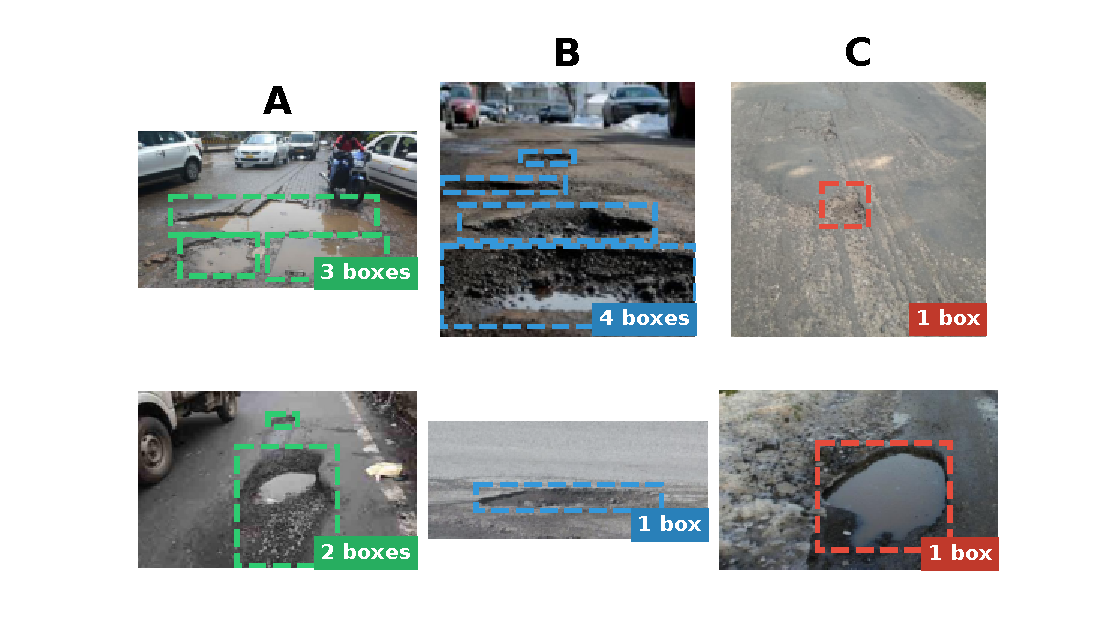
\includegraphics[width=\textwidth]{fig2_dataset_samples.pdf}
   \caption[Representative annotated images from the source repositories.]
           {\label{fig:dataset_samples}Representative annotated images from the
            three source repositories. Ground-truth annotations are shown in
            green (\texttt{chitholian}), blue (\texttt{andrewmvd}) and red
            (\texttt{ashishkumarak}).}
\end{figure}

Three properties of the corpus bear directly on the architectural design of
Chapter~\ref{ch:method}. First, potholes occupy a small and highly variable
fraction of the image area, which is the condition under which multi-scale
feature fusion matters and therefore the condition under which a recalibration
applied at the fusion stage can be expected to have leverage. Second, the
defect boundary is frequently weak: the transition from intact pavement to
defect is gradual, textural rather than photometric, and often partly occluded
by water or debris, so channel-level discrimination between defect texture and
pavement texture is a plausible locus of improvement. Third, the confounders
are spatially structured (shadows, patches and wet regions are contiguous
areas with definite boundaries, not noise) which is the condition under
which spatial attention is a plausible remedy. These three observations are
the empirical basis for combining a channel and a spatial mechanism rather than
either alone.

\section{Threats to Validity}
\label{sec:dataset_threats}

Four properties of the corpus limit what can be concluded from it.

\textbf{Scale.} At 926 images and 2,354 instances the corpus is small by the
standards of general object detection and small even by the standards of the
road-damage benchmarks discussed in Chapter~\ref{ch:related}. The 186-image
validation partition in particular is small enough that individual images
influence the reported metrics measurably, which is the principal reason that
run-to-run variation is comparable in magnitude to the architectural effects
under study.

\textbf{Condition coverage.} All three repositories consist predominantly of
daylight, fair-weather photography. Night, heavy rain, snow, fog and low sun
angles are essentially absent. Frnda et al.~\parencite{frnda2024analysis} show
that detection accuracy degrades sharply and unevenly under exactly these
conditions, so no claim made here extends to them.

\textbf{Viewpoint and geography.} The images are predominantly ground-level
views from vehicle or pedestrian height. Aerial and UAV perspectives, of the
kind represented in UAV-PDD2023 \parencite{pan2025realtime}, are absent, and
the geographic distribution of the source repositories is neither documented
nor controlled.

\textbf{Annotation consistency.} The three repositories were annotated
independently, by different people, without a shared written definition of
what constitutes a pothole or where its boundary lies. Deduplication removed
the redundancy between repositories but cannot reconcile differences in
annotation convention among the images that remain. Some of the residual error
of every model evaluated here is therefore annotation noise rather than
detection failure, and this contributes equally to all configurations.


%%%%%%%%%%%%%%%%%%%%%%%
% CHAPTER 5 -- Attention Design and Training Protocol
%%%%%%%%%%%%%%%%%%%%%%%

\chapter{Attention Design and Training Protocol}
\label{ch:method}

This chapter presents RGDA-YOLOv8m. It begins with the design rationale (the reasoning that determined where attention is applied, which mechanisms are
combined, and why the combination is gated) because those decisions, rather
than the modules themselves, constitute the contribution. It then specifies the
two attention mechanisms mathematically, defines the combined residual-gated
block, accounts for its parameter cost exactly, describes the forward-hook
injection mechanism, and sets out the two-phase training protocol and the
factorial ablation design.

Figure~\ref{fig:pipeline} shows the complete architecture and training
workflow, and serves as a map for the rest of the chapter. A $640 \times 640$
road image enters the C2f-based YOLOv8m backbone, which produces multiscale P3,
P4 and P5 features. The PAN-FPN neck fuses these through top-down and bottom-up
paths, and the three highlighted neck blocks, with channel dimensions
$C \in \{192, 384, 576\}$, are the forward-hook injection points. At each, ECA
performs channel recalibration, CBAM applies its channel and spatial gates, and
the refined tensor is combined with the original through the zero-initialised
residual gate before being passed to the decoupled detection head. The lower
part of the figure summarises the two-phase schedule of
Section~\ref{sec:training}: the backbone is frozen in Phase 1 and all layers
fine-tuned in Phase 2.

\begin{figure}[tbp]
   \centering
   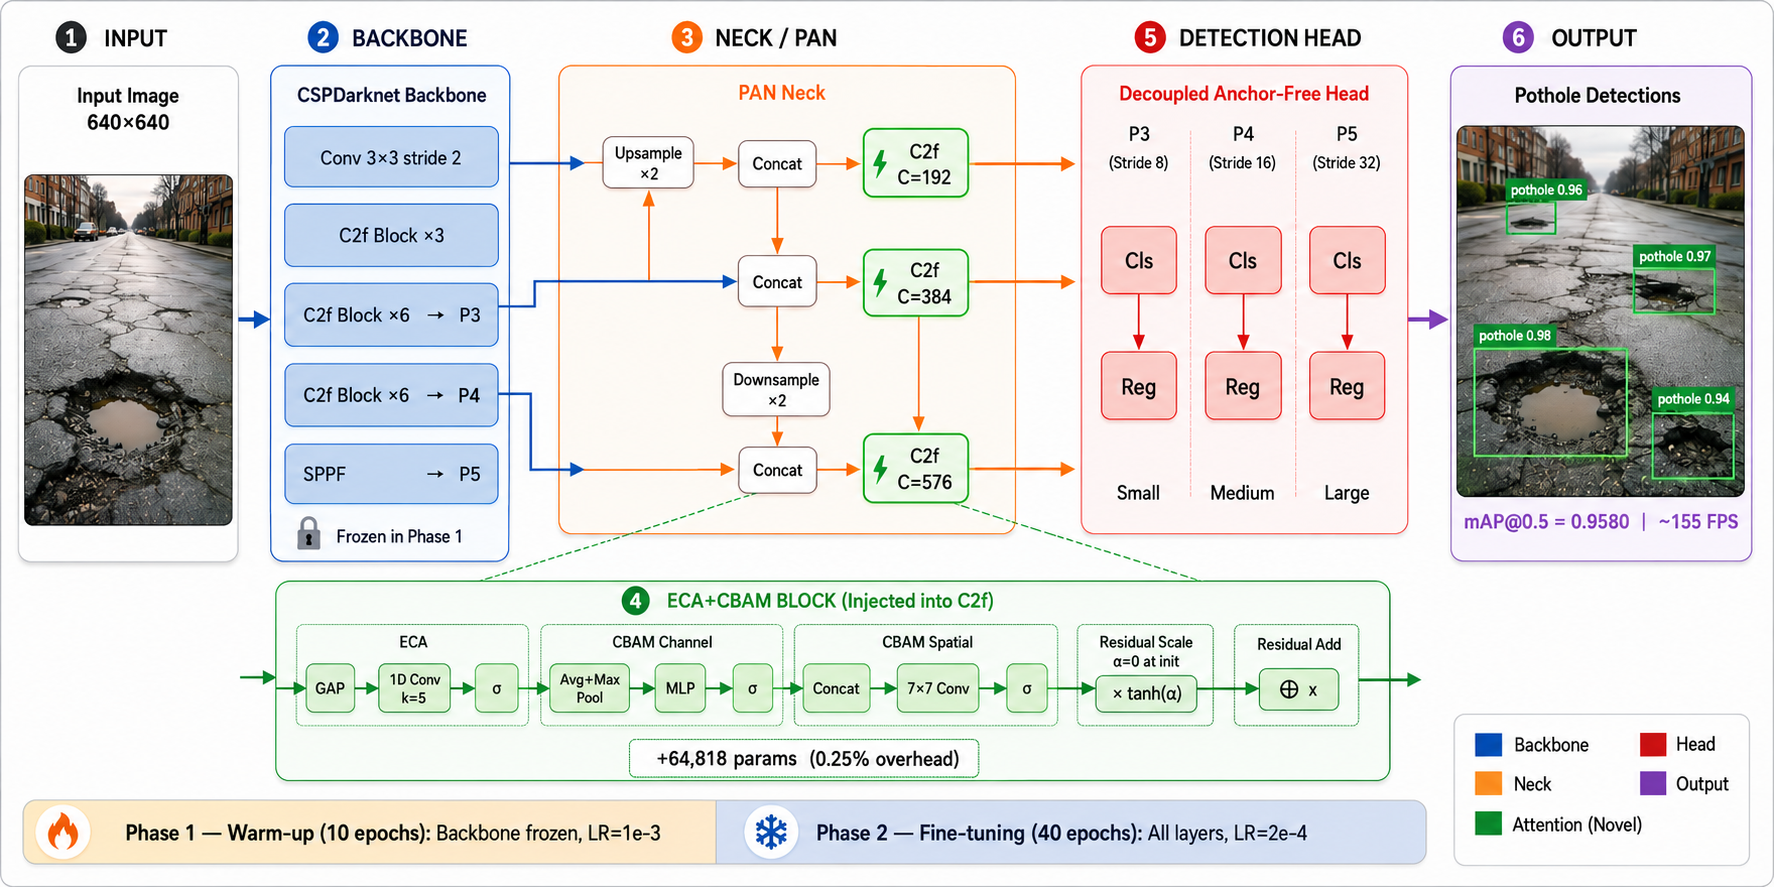
\includegraphics[width=\textwidth]{fig1_pipeline.png}
   \caption[Architecture and training workflow of RGDA-YOLOv8m.]
           {\label{fig:pipeline}Architecture and training workflow of
            RGDA-YOLOv8m. The three highlighted PAN-FPN neck blocks, with
            $C \in \{192, 384, 576\}$, are the forward-hook injection points at
            which the residual-gated ECA--CBAM block is applied.}
\end{figure}

\section{Design Rationale}
\label{sec:rationale}

\subsection{Where to Apply Attention}

An attention module can be inserted almost anywhere in a detector, and the
choice is consequential. Three candidate locations were considered.

Applying attention \emph{within the backbone} would recalibrate features
during extraction, before any multi-scale fusion. This is where several
published road-damage detectors place it
\parencite{chen2024lrsyolo,zhang2025automatic}. The objection in this setting
is that the backbone carries COCO-pretrained weights that constitute most of
the model's transferable knowledge, and that perturbing its intermediate
representations early in fine-tuning on 740 images risks damaging that
knowledge faster than the small dataset can rebuild it.

Applying attention \emph{within the detection head} would recalibrate features
immediately before prediction. The objection is one of leverage: the head
operates on features that are already scale-specialised, so a recalibration
there can only reweight what the neck has already decided to pass on.

Applying attention \emph{at the neck outputs}, the position adopted, places
it at the point where multi-scale information has been fused but before any
prediction has been formed. This is where the representation is richest and
where a reweighting therefore has the widest influence: it affects every
prediction made at that scale. It is also where the confounders identified in
Section~\ref{sec:dataset_stats} are most likely to be separable, because the
fused representation contains both the fine texture cues that distinguish
defect from pavement and the coarse contextual cues that distinguish a defect
from a shadow.

Attention is applied at all three neck outputs rather than a subset, and the
same configuration is used at each. This is a deliberate constraint: it means
the ablation of Section~\ref{sec:ablation_design} varies the \emph{type} of
attention while holding its \emph{position} fixed, so any observed difference
cannot be attributed to placement.

\subsection{Which Mechanisms to Combine}

Section~\ref{sec:dataset_stats} identified two distinct failure modes in this
data. Potholes are confused with visually similar road textures (patched
asphalt, coarse aggregate, wet surfaces) which is a discrimination problem in
the channel dimension, since different channels of a fused feature map respond
to different textural and photometric properties. Potholes are also confused
with spatially structured confounders (shadows, drainage features, worn lane
markings) which is a discrimination problem in the spatial dimension.

A channel mechanism alone can suppress an uninformative feature type but cannot
express that the feature is informative in one part of the image and not
another. A spatial mechanism alone can emphasise a region but operates on
whatever channel mixture it is given, including uninformative channels. The
hypothesis motivating this design is that neither is sufficient in isolation
for this task and that their composition is: suppressing an uninformative
channel helps only if the spatially relevant region is also emphasised, and
emphasising a region helps only if the channels describing it are the
informative ones. This hypothesis is directly testable, and
Section~\ref{sec:ablation_design} sets out the factorial design that tests it.

ECA \parencite{wang2020eca} was selected for the channel stage in preference to
Squeeze-and-Excitation because it avoids the dimensionality-reduction
bottleneck and costs a handful of parameters rather than thousands. CBAM
\parencite{woo2018cbam} was selected for the second stage because it supplies
the spatial mechanism. CBAM contains a channel branch of its own, so placing
ECA before it is not a redundancy but a specific design choice: the ECA factor
in this architecture measures the contribution of an additional,
parameter-light, local cross-channel interaction applied \emph{before} CBAM's
own bottlenecked channel gate and its spatial refinement. This is stated
explicitly because it determines how the ablation must be interpreted.

\subsection{Why the Pathway Is Gated}

A newly attached attention module has randomly initialised weights. On its
first forward pass it therefore multiplies a carefully pretrained feature map
by an arbitrary pattern of values in $(0,1)$, and the resulting gradients
propagate into the backbone and neck. On a large dataset this is survivable.
On 740 images it is a genuine risk: the pretrained representation can be
degraded during the first few hundred optimisation steps faster than the
available data can restore it, and the resulting model may be worse than the
one that was modified.

The remedy adopted is a learnable scalar gate initialised so that the modified
network is, at initialisation, exactly the unmodified network. The attention
pathway then contributes only to the extent that gradient descent finds it
useful to open the gate. This is the same principle that motivates
zero-initialised residual scaling in deep network training
\parencite{bhojanapalli2021zeroinit} and zero-initialised control branches in
conditional generative models \parencite{zhang2023addingcontrol}: a new
component should begin as an identity and earn its influence.

The gate has a second, methodological virtue. Because the modified model at
initialisation is provably identical to the baseline, any difference in final
performance is attributable to what training did with the attention pathway
rather than to a different starting point. Without the gate, the modified and
unmodified runs would begin from different functions, and the comparison would
be correspondingly weaker.

\subsection{Alternatives Considered and Rejected}

Three alternatives were considered. A \emph{fixed} residual weight, such as
$\mathbf{out} = \mathbf{x} + \lambda(\mathrm{Att}(\mathbf{x}) - \mathbf{x})$
with $\lambda$ a hyperparameter, would introduce a constant requiring tuning on
a validation set already being used for reporting. A \emph{per-channel} gate
would allow the network to admit attention selectively by channel, but adds
$C$ parameters per module and, more importantly, makes the initialisation
argument harder to state cleanly. A \emph{parallel} rather than sequential
arrangement of the channel and spatial mechanisms, in the manner of BAM
\parencite{park2018bam}, was not pursued because the sequential arrangement is
what CBAM specifies and changing it would confound the comparison with the
CBAM-only ablation condition. The single scalar gate was retained as the
minimal device that achieves the required property.

\section{Efficient Channel Attention}
\label{sec:eca}

ECA \parencite{wang2020eca} produces one multiplicative weight per channel from
a global descriptor of that channel and its neighbors. For a feature map
$\mathbf{X} \in \mathbb{R}^{C \times H \times W}$, global average pooling
produces a channel descriptor $\mathbf{z} \in \mathbb{R}^{C}$:

\begin{equation}
   z_c \;=\; \frac{1}{HW}\sum_{i=1}^{H}\sum_{j=1}^{W} X_c(i,j).
   \label{eq:eca_pool}
\end{equation}

The descriptor is treated as a one-dimensional signal of length $C$ and
convolved with a single learned kernel of size $k$, after which a sigmoid maps
the result to multiplicative weights:

\begin{equation}
   \mathbf{a} \;=\; \sigma\!\left( \mathrm{Conv1D}_{k}(\mathbf{z}) \right),
   \qquad
   \widehat{\mathbf{X}}_c \;=\; a_c \, \mathbf{X}_c .
   \label{eq:eca_weights}
\end{equation}

Each channel's weight therefore depends on its own descriptor and those of the
$k-1$ neighboring channels, which is the ``local cross-channel interaction''
that gives the method its name. The kernel size is set adaptively from the
channel dimension, on the reasoning that wider layers require wider
interaction:

\begin{equation}
   k \;=\; \Psi(C) \;=\;
   \left|\, \left\lfloor
      \frac{\log_2 (C)}{\gamma} + \frac{b}{\gamma}
   \right\rfloor \,\right|_{\mathrm{odd}},
   \qquad \gamma = 2, \; b = 1,
   \label{eq:eca_kernel}
\end{equation}

where $|\cdot|_{\mathrm{odd}}$ denotes rounding up to the nearest odd integer so
that the convolution can be symmetrically padded. For the three YOLOv8m neck
injection points, with $C \in \{192, 384, 576\}$, Equation~\eqref{eq:eca_kernel}
yields $k = 5$ in every case. Each ECA module therefore contains five learned
parameters, and the three together contain fifteen.

The absence of a bottleneck is the substantive difference from
Squeeze-and-Excitation \parencite{hu2018squeeze}, whose two fully connected
layers with reduction ratio $r$ contain $2C^{2}/r$ parameters, 4,608 at
$C = 192$ against ECA's five, and with every channel interaction forced through
a $C/r$-dimensional bottleneck.

\section{Convolutional Block Attention Module}
\label{sec:cbam}

CBAM \parencite{woo2018cbam} refines a feature map in two sequential stages.
Writing $\otimes$ for element-wise multiplication with broadcasting:

\begin{equation}
   \mathbf{F}' = \mathbf{M}_c(\mathbf{F}) \otimes \mathbf{F},
   \qquad
   \mathbf{F}'' = \mathbf{M}_s(\mathbf{F}') \otimes \mathbf{F}' .
   \label{eq:cbam_seq}
\end{equation}

The channel gate $\mathbf{M}_c \in \mathbb{R}^{C \times 1 \times 1}$ extends
Squeeze-and-Excitation by summing the responses of a shared two-layer
perceptron to both average-pooled and max-pooled descriptors, on the reasoning
that average pooling captures the extent of a response while max pooling
captures its peak:

\begin{equation}
\begin{split}
   \mathbf{M}_c(\mathbf{F}) = \sigma\bigl(&
      \mathrm{MLP}(\mathrm{AvgPool}(\mathbf{F})) \\
      &+ \mathrm{MLP}(\mathrm{MaxPool}(\mathbf{F})) \bigr).
\end{split}
\label{eq:cbam_channel}
\end{equation}

The perceptron is implemented as two $1 \times 1$ convolutions with a
ReLU between them, reducing to $C/r$ channels and restoring to $C$, with
reduction ratio $r = 16$ throughout this work.

The spatial gate $\mathbf{M}_s \in \mathbb{R}^{1 \times H \times W}$ pools
across the channel dimension rather than the spatial one, producing two
single-channel maps that are concatenated and convolved:

\begin{equation}
   \mathbf{M}_s(\mathbf{F}) = \sigma\!\left(
      f^{7 \times 7}\!\left[
         \mathrm{AvgPool}_{c}(\mathbf{F}); \,
         \mathrm{MaxPool}_{c}(\mathbf{F})
      \right] \right).
   \label{eq:cbam_spatial}
\end{equation}

The $7 \times 7$ kernel is deliberately large: the spatial gate must decide
whether a region is a defect or a confounder, and that decision requires
context beyond the immediate neighborhood.

\section{The Residual-Gated ECA--CBAM Block}
\label{sec:rgda_block}

\subsection{Composition}

The proposed block applies ECA, then CBAM's channel gate, then CBAM's spatial
gate, and combines the result with the untransformed input through a learnable
scalar gate. Writing $\mathrm{A}(\mathbf{x})$ for the composed attention
transformation,

\begin{equation}
   \mathrm{A}(\mathbf{x}) \;=\;
      \mathbf{M}_s(\mathbf{u}) \otimes \mathbf{u},
   \qquad
   \mathbf{u} \;=\; \mathbf{M}_c(\mathbf{e}) \otimes \mathbf{e},
   \qquad
   \mathbf{e} \;=\; \mathrm{ECA}(\mathbf{x}),
   \label{eq:composed}
\end{equation}

the block output is

\begin{equation}
   \boxed{\;
   \mathbf{out} \;=\; \mathbf{x} \;+\;
      \tanh(\alpha) \left[ \mathrm{A}(\mathbf{x}) - \mathbf{x} \right],
   \;}
   \label{eq:residual}
\end{equation}

where $\alpha \in \mathbb{R}$ is a single learnable parameter initialised to
zero.

Figure~\ref{fig:attention_block} shows the internal structure.

\begin{figure}[tbp]
   \centering
   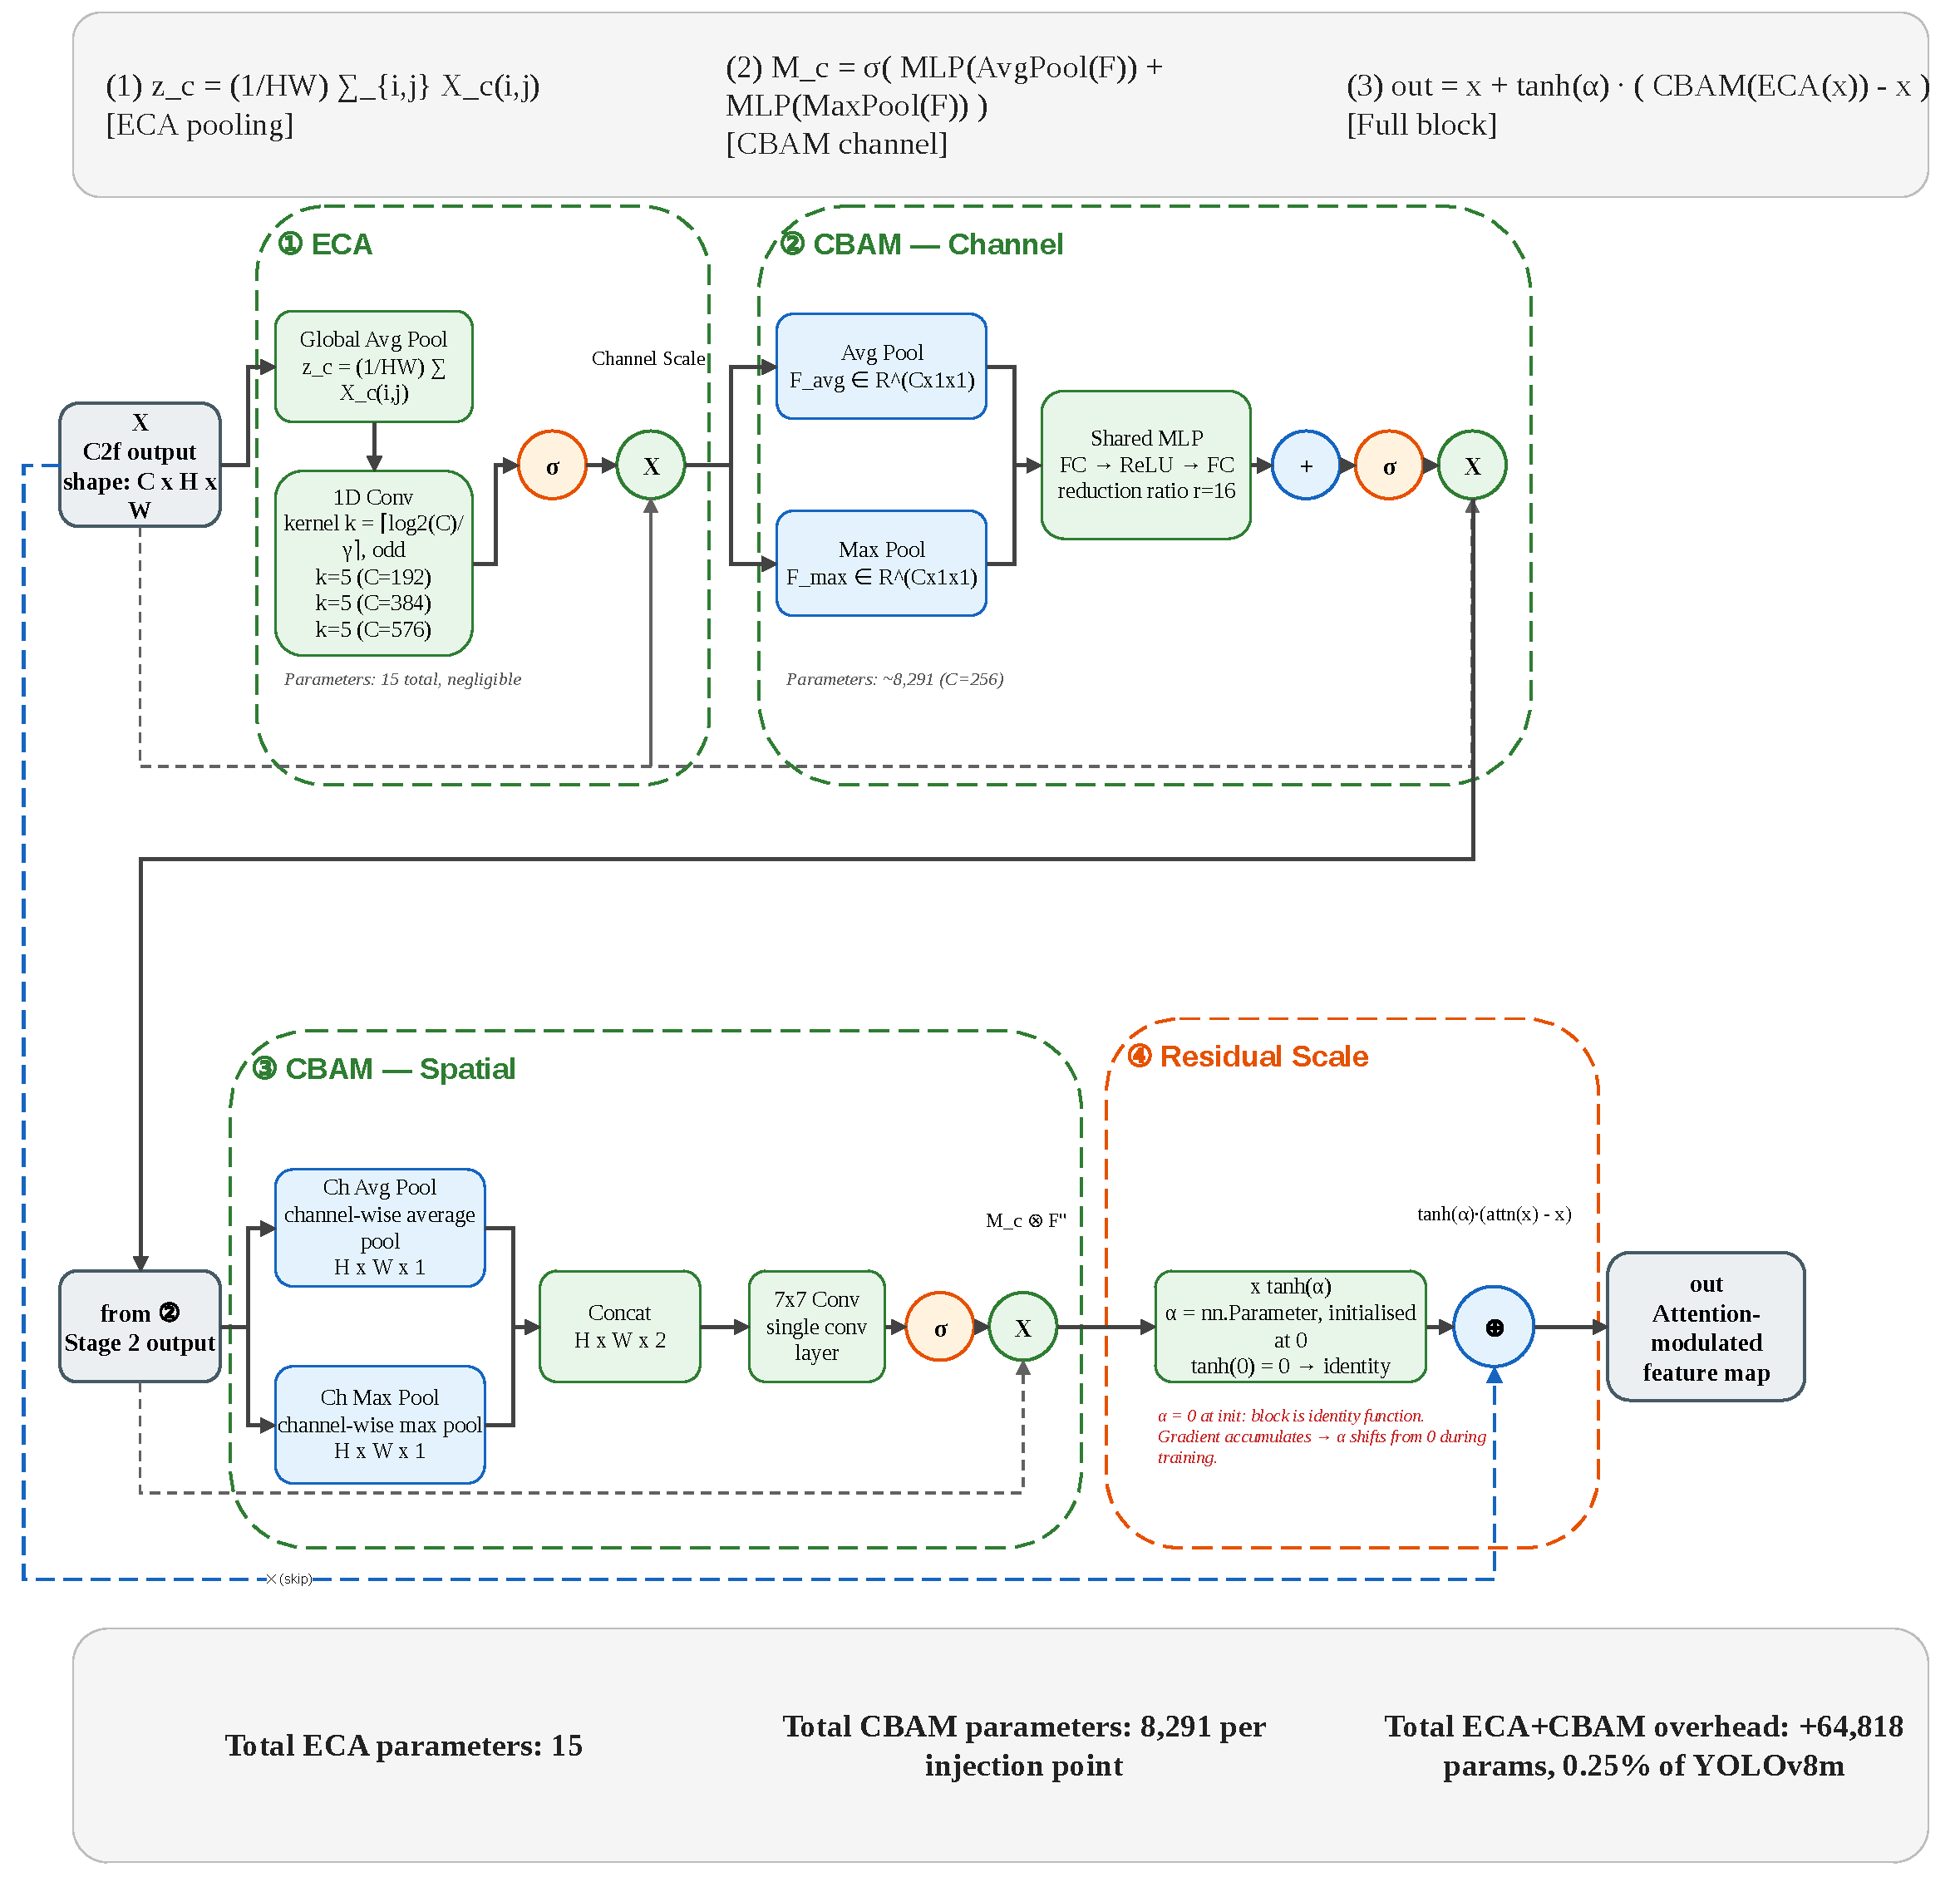
\includegraphics[width=0.72\textwidth]{fig3_attention_block.drawio.pdf}
   \caption[The residual-gated ECA--CBAM block.]
           {\label{fig:attention_block}The residual-gated ECA--CBAM block. The
            input passes through ECA channel recalibration, then CBAM's channel
            and spatial gates. The refined output is combined with the
            unmodified input through the learnable gate $\alpha$, initialised
            to zero.}
\end{figure}

\subsection{Properties of the Gate}

Equation~\eqref{eq:residual} is written as an interpolation rather than as a
plain residual sum for a specific reason. Because $\tanh(0) = 0$, at
initialisation

\begin{equation}
   \mathbf{out} \;=\; \mathbf{x} + 0 \cdot
      \left[ \mathrm{A}(\mathbf{x}) - \mathbf{x} \right]
   \;=\; \mathbf{x},
\end{equation}

so the modified detector computes exactly the same function as the pretrained
one. Had the block been written as $\mathbf{x} + \tanh(\alpha)\mathrm{A}(\mathbf{x})$,
zero initialisation would give $\mathbf{out} = \mathbf{x}$ as well, but the
gate would then interpolate between the identity and the identity-plus-attention
rather than between the identity and attention itself, and $\tanh(\alpha) = 1$
would double the feature magnitude. The interpolation form makes
$\tanh(\alpha) = 1$ correspond to full attention and $\tanh(\alpha) = 0$ to
none, which is the intended semantics.

The $\tanh$ envelope bounds the gate to $(-1, 1)$, which prevents the optimiser
from driving the attention contribution to an arbitrarily large magnitude and
destabilising training, a real possibility given that $\alpha$ is a single
unregularised scalar receiving gradient from every spatial position of every
channel. The negative half of the range is available and meaningful: it allows
the network to apply the attention correction in the opposite direction if that
is what reduces the loss.

The gradient with respect to $\alpha$ is

\begin{equation}
   \frac{\partial \mathcal{L}}{\partial \alpha}
   = \bigl(1 - \tanh^{2}(\alpha)\bigr)
     \left\langle
        \frac{\partial \mathcal{L}}{\partial \mathbf{out}},\;
        \mathrm{A}(\mathbf{x}) - \mathbf{x}
     \right\rangle,
   \label{eq:alpha_grad}
\end{equation}

which is maximal at $\alpha = 0$ and vanishes as $|\alpha|$ grows. The gate
therefore moves fastest when it is closed, which is the desirable behaviour: it
opens readily if the attention pathway is useful and saturates rather than
diverging if it is.

\subsection{Parameter Accounting}

The block's parameter cost is small and exactly computable.
Table~\ref{tab:params} gives the breakdown at each injection point. Writing
$m = \lfloor C/r \rfloor$ for the CBAM bottleneck width with $r = 16$, each
block contains $k$ parameters for the ECA convolution, $2Cm$ for the two
bias-free $1\times1$ convolutions of the channel gate, $2 \times 7 \times 7 = 98$
for the bias-free spatial convolution, and one for $\alpha$.

\begin{table}[tbp]
\centering
\small
\setlength{\tabcolsep}{4pt}
\begin{tabularx}{\textwidth}{@{}>{\RaggedRight\arraybackslash}X rrrrrr@{}}
\toprule
\textbf{Injection point} & \textbf{$C$} & \textbf{$k$} & \textbf{ECA} &
\textbf{Channel gate} & \textbf{Spatial gate} & \textbf{Total} \\
\midrule
Shallow (P3 fusion) & 192 & 5 & 5  & 4{,}608  & 98 & 4{,}712 \\
Middle (P4 fusion)  & 384 & 5 & 5  & 18{,}432 & 98 & 18{,}536 \\
Deep (P5 fusion)    & 576 & 5 & 5  & 41{,}472 & 98 & 41{,}576 \\
\midrule
\textbf{Total}      & --- & --- & \textbf{15} & \textbf{64{,}512} &
   \textbf{294} & \textbf{64{,}824} \\
\bottomrule
\end{tabularx}
\caption[Parameter cost of the residual-gated block.]
        {\label{tab:params}Parameter cost of the residual-gated ECA--CBAM block
         at each of the three neck injection points. Each row includes one
         parameter for the gate $\alpha$. The total of 64,824 parameters
         represents a 0.25 percent increase over the 25.9-million-parameter
         YOLOv8m base model.}
\end{table}

Two features of this accounting are worth noting. The channel gate accounts for
99.5 percent of the added parameters, because its cost grows as $C^{2}/r$ while
the other components are constant or logarithmic in $C$. And the deep injection
point alone accounts for 64 percent of the total, for the same reason. The
entire mechanism costs 0.25 percent of the base model, which places any
observed improvement in a different category from one obtained by scaling the
model up.

\section{Hook-Based Neck Injection}
\label{sec:injection}

\subsection{Layer Selection}

The injector locates candidate blocks by scanning the detector's top-level
module sequence for blocks whose class name belongs to
$\{\texttt{C3k2}, \texttt{C2f}, \texttt{C2fAttn}, \texttt{RepC3}, \texttt{C3}\}$.
This set spans the fusion block types used across the YOLO versions under
study, which is what allows the identical injector to be applied to both
YOLOv8m and YOLOv11m in Section~\ref{sec:results_saturation} without
modification, a necessary condition for that comparison to be controlled.

Blocks of these types occur in both the backbone and the neck. The selection
rule retains the \emph{last three} matches. This is correct because the
Ultralytics model sequence is ordered from input to output: backbone blocks
necessarily precede neck blocks, and the three PAN-FPN fusion blocks that feed
the detection head are the final three matches in the sequence. The rule is
positional rather than name-based, which makes it robust to the naming
differences between YOLO versions.

\subsection{Channel Probing}

The number of output channels of each selected block is determined empirically
rather than assumed. Temporary probe hooks are registered on the three
candidate blocks, a dummy tensor is passed through the model, each probe
records the channel dimension of the tensor its block emitted, and the probes
are removed. The recorded dimensions (192, 384 and 576 for YOLOv8m) are
then used to construct correctly sized attention modules.

This step exists because block output width depends on the model scale
multipliers, which differ between the n, s, m, l and x variants of each YOLO
version. Hard-coding the widths would silently produce a shape mismatch, or
worse a silently incorrect module, on any variant other than the one the
constants were written for. Probing makes the injector correct by construction
across scales and versions.

\subsection{The Hook}

A forward hook is then registered on each selected block. When the block
returns, the hook receives its output tensor, applies the residual-gated
transformation of Equation~\eqref{eq:residual}, and returns the result, which
PyTorch substitutes for the original output before it reaches the next module.
Where a block returns a tuple rather than a tensor, the hook transforms the
first element and reconstructs the tuple.

\subsection{Consequences of the Mechanism}

The advantage of this mechanism was stated in
Section~\ref{sec:framework}: the model definition, layer indices and framework
source are untouched, so the modified and unmodified configurations are
identical in every respect except the transformation applied at three points.

One further implementation detail is necessary for the mechanism to work at
all. Registering the hooks on the model object before invoking Ultralytics
training has no effect, because \texttt{YOLO.train()} constructs its own
\texttt{nn.Module} for the trainer and only reassigns it onto the model object
after training completes. The hooked object is therefore discarded the moment
training begins. The failure is silent, every configuration trains and
evaluates successfully and every configuration reproduces the unmodified
baseline, which is easily misread as the attention mechanism having no
effect. The hooks are consequently attached from an \texttt{on\_train\_start}
callback, which fires after the live trainer model has been built. This is
documented here because the same trap would affect any attempt to reproduce or
extend this work.

The cost is that the attention parameters live outside the detector's module
tree and therefore outside its \texttt{state\_dict}. They must be persisted
separately by the training pipeline and reattached explicitly before inference.
A checkpoint written by Ultralytics and loaded without the accompanying
attention state produces an unmodified YOLOv8m that runs without error and
reports plausible results, which is a failure mode that is silent rather than
loud. This is the principal implementation limitation of the work and is
revisited in Section~\ref{sec:disc_limitations}.

\section{Two-Phase Training Protocol}
\label{sec:training}

\subsection{Motivation}

Fine-tuning a COCO-pretrained detector on 740 domain-specific images with newly
attached, randomly initialised modules poses a scheduling problem. Training
everything at once at a learning rate high enough to adapt the new modules
risks disturbing the pretrained backbone. Training at a rate low enough to
protect the backbone leaves the new modules undertrained. The protocol adopted
separates these concerns in time.

\subsection{Phase 1: Backbone Stabilisation}

The first ten layers of the detector are frozen, and the attention modules
together with the remaining layers and the detection head are trained for ten
epochs at an initial learning rate of $1 \times 10^{-3}$ with weight decay
$5 \times 10^{-4}$. Freezing the early backbone protects the general-purpose
low-level features that transfer well from COCO, while allowing the head to
adapt to a single-class problem with a very different object-scale distribution
from the pretraining data.

\subsection{Phase 2: Full-Model Fine-Tuning}

The best checkpoint from Phase 1 is loaded into a fresh \texttt{YOLO} object, a
newly initialised attention module is attached at the same three locations, all
layers are unfrozen, and training continues for forty epochs at a reduced
initial learning rate of $2 \times 10^{-4}$. The reduction by a factor of five
reflects that the model now begins from a domain-adapted rather than a
COCO-pretrained state, and that the backbone is no longer protected by
freezing.

Table~\ref{tab:training} summarises both phases.

\begin{table}[tbp]
\centering
\small
\begin{tabular}{@{}lcc@{}}
\toprule
\textbf{Parameter} & \textbf{Phase 1} & \textbf{Phase 2} \\
\midrule
Epochs                & 10 & 40 \\
Initial learning rate & $1 \times 10^{-3}$ & $2 \times 10^{-4}$ \\
Batch size            & 16 & 16 \\
Input resolution      & $640 \times 640$ & $640 \times 640$ \\
Frozen layers         & 10 & 0 \\
Data-loader workers   & 2 & 2 \\
Weight decay          & $5 \times 10^{-4}$ & $5 \times 10^{-4}$ \\
Attention module      & $\phi_1$ (discarded) & $\phi_2$ (retained) \\
\bottomrule
\end{tabular}
\caption[Two-phase training configuration.]
        {\label{tab:training}Two-phase training configuration for
         RGDA-YOLOv8m. The same schedule was applied to the YOLOv8m+CBAM and
         YOLOv8m+CoordAttn comparators and to every cell of the ablation, so
         that differences between them reflect the attention configuration
         rather than the optimisation settings.}
\end{table}

\subsection{Why the Phase-1 Attention Module Is Discarded}

A fresh \texttt{YOLO} object is instantiated for Phase 2 to avoid trainer-state
conflicts that arise when Ultralytics training is invoked twice on the same
object. Because the attention parameters are external to the checkpoint, as
Section~\ref{sec:injection} explained, they do not survive that reload: the
Phase-1 module $\phi_1$, including its learned gate $\alpha$, is discarded, and
a new module $\phi_2$ with $\alpha = 0$ is attached for Phase 2.

The consequence should be stated plainly rather than glossed. Phase 1 does not
pre-train the attention pathway. What it produces is a set of backbone and head
parameters that have been adapted to the pothole domain \emph{under an
attention-modulated training loss}, and Phase 2 trains a new attention module
jointly with that adapted detector from a closed gate. The protocol is
therefore best understood as domain adaptation followed by gated attention
training, not as a two-stage curriculum for the attention module. Whether
carrying $\phi_1$ into Phase 2 would perform better is an open question that
this design does not answer. It is listed as future work in
Section~\ref{sec:future_work}.

\subsection{Comparator Training}

The YOLOv8m+CBAM and YOLOv8m+CoordAttn comparators, and every cell of the
ablation, were trained under exactly this schedule from the same
COCO-pretrained YOLOv8m initialisation. YOLOv8m, YOLOv10m and YOLOv11m
baselines were fine-tuned for 50 epochs at $640 \times 640$ with batch size 16
under Ultralytics automatic optimiser selection with \texttt{lr0=0.01}. RT-DETR
was fine-tuned for 50 epochs at batch size 8 from the \texttt{rtdetr-l.pt}
checkpoint, with automatic selection choosing AdamW at learning rate 0.002 and
momentum 0.9. Faster R-CNN and SSD-VGG16 were fine-tuned for 20 epochs with SGD
at momentum 0.9 and weight decay 0.0005. Faster R-CNN used learning rate 0.005
at batch size 4, while SSD-VGG16 required learning rate 0.0005, batch size 1
and gradient-norm clipping at 1.0 to remain numerically stable. The latter two
were trained without validation-based checkpoint selection, so their
final-epoch weights were retained. These budget differences are a genuine
limitation of the cross-architecture comparison and are treated as such in
Section~\ref{sec:disc_limitations}.

\section{Algorithmic Summary}
\label{sec:algorithms}

Algorithm~\ref{alg:forward} states the forward pass of RGDA-YOLOv8m, including
the residual-gated operation applied at each injection point.
Algorithm~\ref{alg:twophase} states the multi-seed two-phase training
procedure.

\begin{algorithm}[!ht]
\caption{Forward pass of RGDA-YOLOv8m}
\label{alg:forward}
\begin{algorithmic}[1]
\Require Image $I \in \mathbb{R}^{H \times W \times 3}$; detector parameters
         $\boldsymbol{\theta}$; attention parameters $\phi$
\Ensure  Detections $\{(\mathrm{box}_i, \mathrm{class}_i, \mathrm{conf}_i)\}$
\Statex
\Statex \textit{\textbf{Preprocessing}}
\State $I' \gets \mathrm{Normalize}(\mathrm{Resize}(I, 640 \times 640))$
\Statex
\Statex \textit{\textbf{Backbone and neck}}
\State $\{P_3, P_4, P_5\} \gets \mathrm{Backbone}_{\boldsymbol{\theta}}(I')$
   \Comment{C2f multiscale features}
\State $\{N_3, N_4, N_5\} \gets \mathrm{Neck}_{\boldsymbol{\theta}}(P_3, P_4, P_5)$
   \Comment{PAN-FPN fusion}
\Statex
\Statex \textit{\textbf{Residual-gated attention at each neck output}}
\For{each scale $s \in \{3, 4, 5\}$}
   \State $X \gets N_s$
   \State $\mathbf{z} \gets \mathrm{GlobalAvgPool}(X)$
   \State $\boldsymbol{\omega} \gets \sigma(\mathrm{Conv1D}_{k}(\mathbf{z}))$
   \State $X_1 \gets X \otimes \boldsymbol{\omega}$
      \Comment{ECA channel recalibration}
   \State $\mathbf{M}_c \gets \sigma\bigl(
             \mathrm{MLP}(\mathrm{AvgPool}(X_1)) +
             \mathrm{MLP}(\mathrm{MaxPool}(X_1)) \bigr)$
   \State $X_2 \gets X_1 \otimes \mathbf{M}_c$
      \Comment{CBAM channel gate}
   \State $\mathbf{M}_s \gets \sigma\bigl( f^{7\times7}[
             \mathrm{AvgPool}_{c}(X_2); \mathrm{MaxPool}_{c}(X_2)] \bigr)$
   \State $X_3 \gets X_2 \otimes \mathbf{M}_s$
      \Comment{CBAM spatial gate}
   \State $N_s \gets X + \tanh(\alpha_s)\,(X_3 - X)$
      \Comment{gate; $\alpha_s = 0$ at initialisation}
\EndFor
\Statex
\Statex \textit{\textbf{Detection and post-processing}}
\State $R \gets \mathrm{DetectionHead}_{\boldsymbol{\theta}}(N_3, N_4, N_5)$
\State $R \gets \mathrm{ApplyConfidenceThreshold}(R, \tau_{\mathrm{conf}})$
\State \textbf{return} $\mathrm{NonMaxSuppression}(R, 0.45)$
\end{algorithmic}
\end{algorithm}

\begin{algorithm}[!ht]
\caption{Two-phase multi-seed training of RGDA-YOLOv8m}
\label{alg:twophase}
\begin{algorithmic}[1]
\Require Deduplicated corpus $D$; COCO-pretrained $\boldsymbol{\theta}_0$;
         seeds $S = \{42, 123, 456\}$
\Ensure  Trained parameters and aggregated metrics
\State $(D_{\mathrm{train}}, D_{\mathrm{val}}) \gets
        \mathrm{Split}(D, 0.8, \mathrm{seed}=42)$
   \Comment{fixed across all seeds}
\For{each seed $s \in S$}
   \State $\mathrm{SetRandomState}(s)$;\quad
          $\boldsymbol{\theta} \gets \boldsymbol{\theta}_0$
   \Statex \quad\textit{\textbf{Phase 1: backbone stabilisation}}
   \State $\phi_1 \gets \mathrm{AttachAttention}(\boldsymbol{\theta},
           \{N_3, N_4, N_5\})$; freeze the first 10 layers
      \Comment{$\alpha = 0$}
   \State Train $(\boldsymbol{\theta}_{\mathrm{unfrozen}}, \phi_1)$ for 10
          epochs at $\mathrm{lr}_0 = 1{\times}10^{-3}$
   \State $\boldsymbol{\theta}_1 \gets$ best-validation checkpoint;\quad
          discard $\phi_1$
   \Statex \quad\textit{\textbf{Phase 2: full-model fine-tuning}}
   \State Instantiate a fresh detector from $\boldsymbol{\theta}_1$;\quad
          $\phi_2 \gets \mathrm{AttachAttention}(\boldsymbol{\theta}_1,
          \{N_3, N_4, N_5\})$
      \Comment{$\alpha = 0$ again}
   \State Unfreeze all layers and train $(\boldsymbol{\theta}, \phi_2)$ for 40
          epochs at $\mathrm{lr}_0 = 2{\times}10^{-4}$
   \State $M_s \gets \mathrm{Evaluate}(\boldsymbol{\theta}, \phi_2,
           D_{\mathrm{val}})$; persist $\boldsymbol{\theta}$, $\phi_2$ and
           $M_s$ to disk
\EndFor
\State \textbf{return} $\mathrm{mean}(M_s)$, $\mathrm{std}(M_s)$ over $s \in S$
\end{algorithmic}
\end{algorithm}

\section{Ablation Design}
\label{sec:ablation_design}

The hypothesis of Section~\ref{sec:rationale}, that neither the channel nor
the spatial mechanism is sufficient alone and that the effect belongs to their
combination, is tested by a $2 \times 2$ factorial design over the presence
of ECA and the presence of CBAM, giving the four conditions of
Table~\ref{tab:factorial}.

\begin{table}[htbp]
\centering
\small
\begin{tabular}{@{}lcc@{}}
\toprule
 & \textbf{Without CBAM} & \textbf{With CBAM} \\
\midrule
\textbf{Without ECA} & Baseline (no attention) & CBAM-only \\
\textbf{With ECA}    & ECA-only                & ECA+CBAM (proposed) \\
\bottomrule
\end{tabular}
\caption[Factorial ablation design.]
        {\label{tab:factorial}The $2 \times 2$ factorial ablation over the
         presence of the channel and channel--spatial pathways. All four
         conditions share the dataset partition, injection points, gate,
         training schedule, confidence threshold and IoU threshold.}
\end{table}

All four conditions use the same partition, the same three injection points,
the same zero-initialised gate, the same two-phase schedule, the same
confidence threshold of 0.25 and the same IoU threshold of 0.5. The only
difference is which transformation the gate interpolates towards. Each
condition is run at all three seeds and reported as a mean with standard
deviation.

Because CBAM contains a channel branch of its own
(Equation~\eqref{eq:cbam_channel}), the ECA factor does not measure the
contribution of channel attention in general. It measures the contribution of
an \emph{additional}, parameter-light, local cross-channel interaction applied
before CBAM's bottlenecked channel gate. A reader interpreting the ablation as
``channel attention versus spatial attention'' would draw the wrong conclusion
from it, which is why the point is made here as well as in
Chapter~\ref{ch:results}.


%%%%%%%%%%%%%%%%%%%%%%%
% CHAPTER 6 -- Evaluation Metrics and Measurement Protocol
%%%%%%%%%%%%%%%%%%%%%%%

\chapter{Evaluation Metrics and Measurement Protocol}
\label{ch:metrics}

Chapter~\ref{ch:related} argued that published road-defect detection results
are frequently incomparable because the procedures that produced them are
unstated. This chapter specifies, for this dissertation, every choice that
affects a reported number: how predictions are matched to ground truth, how
precision, recall, F1 and average precision are computed, at which operating
points they are reported, how throughput is measured, and how variation across
training runs is characterised. The purpose is to make the results of
Chapter~\ref{ch:results} reproducible and to make explicit which comparisons
they support.

\section{Matching Predictions to Ground Truth}
\label{sec:matching}

Every detection metric begins with a decision about which predicted boxes count
as correct. Overlap is measured by intersection over union: for a predicted box
$B_p$ and a ground-truth box $B_g$,

\begin{equation}
   \mathrm{IoU}(B_p, B_g)
   \;=\; \frac{|B_p \cap B_g|}{|B_p \cup B_g|} ,
   \label{eq:iou}
\end{equation}

which is one when the boxes coincide, zero when they are disjoint, and
scale-invariant. A prediction is eligible to be a true positive when its IoU
with some ground-truth box is at least 0.5.

Eligibility is not sufficient, because several predictions may overlap the same
annotation. The matching rule used throughout is the greedy one adopted by the
PASCAL VOC and COCO reference implementations
\parencite{everingham2010pascal,lin2014microsoft}. Detections are sorted by
descending confidence. Each detection in turn is assigned to the
highest-IoU ground-truth box that is still unmatched and that meets the
threshold. That box is then removed from consideration. A detection for which
no unmatched ground-truth box meets the threshold is a false positive. A
ground-truth box that remains unmatched when every detection has been processed
is a false negative.

Two properties of this rule matter for interpretation. Confidence ordering means
a lower-scoring detection cannot displace a higher-scoring one from an
annotation, so duplicate detections of the same pothole are counted as false
positives, which is the intended behaviour, since a system that reports one
defect three times is reporting incorrectly. And because each annotation can be
claimed only once, the number of true positives is bounded above by the number
of annotations, so recall is well defined. This identical rule was applied to
every configuration in this study, including those scored outside the
Ultralytics evaluator.

\section{Precision, Recall and F1}
\label{sec:prf}

Given counts of true positives $TP$, false positives $FP$ and false negatives
$FN$:

\begin{align}
   \mathrm{Precision} &= \frac{TP}{TP + FP}, &
   \mathrm{Recall}    &= \frac{TP}{TP + FN}, \notag \\[4pt]
   \mathrm{F1}        &= \frac{2 \cdot \mathrm{Precision} \cdot \mathrm{Recall}}
                              {\mathrm{Precision} + \mathrm{Recall}} .
   \label{eq:prf}
\end{align}

For this application the two error types have different practical costs, and
neither dominates. A false negative is an unreported hazard: a pothole that a
maintenance survey misses, or a defect an assistive system fails to warn about.
A false positive is a wasted inspection or, in the assistive case, a spurious
alert. A system that alerts on every shadow will be switched off, at which
point its recall becomes irrelevant. F1, as their harmonic mean, penalises a
detector that achieves a high value of one by sacrificing the other, and is
therefore the single-number summary reported here alongside mAP.

\section{Average Precision}
\label{sec:ap}

\subsection{The Precision--Recall Curve}

Precision and recall as defined above describe a detector at one confidence
threshold. Sweeping the threshold from high to low traces a
precision--recall curve: at a high threshold few detections are emitted, so
precision is typically high and recall low. As the threshold falls, recall
rises and precision generally falls. Average precision summarises the whole
curve and is therefore threshold-independent, which is why it is the primary
metric for comparing detectors.

\subsection{Interpolation and Integration}

The raw curve is not monotone, admitting one more detection can raise
precision if it is correct, so it is first replaced by its monotonically
non-increasing envelope:

\begin{equation}
   p_{\mathrm{env}}(r) \;=\; \max_{r' \geq r} p(r') .
   \label{eq:envelope}
\end{equation}

Average precision is then the area under that envelope:

\begin{equation}
   \mathrm{AP} \;=\; \int_{0}^{1} p_{\mathrm{env}}(r) \, \mathrm{d}r ,
   \label{eq:ap}
\end{equation}

and mean average precision is the mean of $\mathrm{AP}_c$ over classes
$c \in \mathcal{C}$. This corpus contains a single class, so mAP@0.5 equals
$\mathrm{AP}$ at an IoU threshold of 0.5. The notation is retained for
consistency with the literature. Where reported, mAP@0.5:0.95 is the mean of
$\mathrm{AP}$ computed at IoU thresholds from 0.50 to 0.95 in steps of 0.05,
which rewards precise localisation rather than mere detection.

\subsection{Which Interpolation Rule}

Equation~\eqref{eq:ap} is evaluated by trapezoidal integration over 101
uniformly spaced recall values in $[0, 1]$, which is the COCO convention
\parencite{lin2014microsoft} and the definition implemented by Ultralytics
\texttt{model.val()}. It is not the only convention in use. The PASCAL VOC 2007
rule averages interpolated precision at eleven recall levels
$\{0, 0.1, \ldots, 1.0\}$ \parencite{everingham2010pascal}, and yields
systematically different values from the same predictions.

The difference is not negligible. Scoring the same YOLOv11m+ECA+CBAM
predictions under both rules gives a mean mAP@0.5 of 0.7555 under the VOC
11-point rule and 0.7823 under COCO 101-point interpolation, a gap of 2.7
percentage points, more than three times the size of the architectural effect
this dissertation sets out to measure. A paper reporting ``mAP@0.5'' without
stating the rule has therefore left its reader unable to compare its number
with anyone else's. The COCO rule is used exclusively here, and applied
identically to every configuration.

That last point requires enforcement rather than assertion. Four configurations (Faster R-CNN, SSD-VGG16, RT-DETR and the WBF ensemble) are not scored by
\texttt{model.val()} but by a custom evaluator, because they are either not
Ultralytics models or, in the ensemble's case, not a model at all. That
evaluator implements Equations~\eqref{eq:iou} to \eqref{eq:ap} directly, so its
outputs are commensurable with those of \texttt{model.val()}.

Two boundary conventions complete the specification. Precision--recall curves
are generated from detections produced at a confidence threshold of 0.001, so
that integration covers the full curve rather than a truncated segment of it. A
higher threshold would silently discard the low-precision, high-recall tail and
inflate AP. And a configuration for which no detection survives the threshold
is assigned $\mathrm{AP} = 0$ rather than having Equation~\eqref{eq:ap}
evaluated from boundary conditions, which would otherwise produce an
artificially non-zero value from an empty curve.

\subsection{Why mAP@0.5 Is the Primary Metric}

Two IoU regimes are reported in this dissertation, and their roles differ.
mAP@0.5 asks whether the detector found the defect. MAP@0.5:0.95 asks
additionally how precisely it delineated it. For general object detection the
stricter metric is usually preferred, because a tight box on a rigid object is
both achievable and useful.

For potholes it is less informative, for the reason given in
Section~\ref{sec:what_makes_hard}: the defect boundary is genuinely gradual, so
where the annotator drew the box is partly a judgement, and the three source
repositories were annotated independently without a shared convention. A metric
that rewards agreement with the annotator's boundary at IoU 0.9 is therefore
partly measuring annotation style. mAP@0.5 is reported as the primary metric
because the downstream tasks (warning a pedestrian, flagging a location for
inspection) require knowing that a defect is present and roughly where, not
its exact extent. mAP@0.5:0.95 is reported alongside it in
Table~\ref{tab:multiseed} so that a reader
interested in localisation quality can see it, and because a change that
improves the loose metric while degrading the strict one would indicate that
the model had learned to emit larger boxes rather than better ones.

\section{Operating Points}
\label{sec:operating_points}

\subsection{The Problem With a Single Threshold}

Precision, recall and F1 require a confidence threshold. Comparing detectors at
a common fixed threshold appears fair and often is not, because detectors
differ in how they distribute confidence. A model whose scores are compressed
towards the top of the range and one whose scores are spread across it will
occupy very different positions on their respective precision--recall curves at
the same numerical threshold, and the resulting F1 comparison will conflate
detection capability with score calibration.

This is not hypothetical in the present study. The F1-maximising threshold
varies between 0.10 and 0.70 across the ten configurations evaluated. A single
fixed threshold therefore places some detectors near their optimum and others
far from it.

\subsection{Two Reported Operating Points}

Two operating points are consequently reported for every configuration.

The first is a \textbf{fixed threshold of 0.25}, applied uniformly. This
represents a deployment setting in which one threshold is chosen and applied
without per-model tuning, and it is the operating point at which precision,
recall and F1 are reported unless stated otherwise.

The second is \textbf{F1$^{\ast}$}, the maximum F1 attained over a sweep of the
confidence threshold across $[0.05, 0.70]$. This characterises the detector at
the best point on its own curve and is therefore independent of calibration.

Reporting both separates two questions that a single number conflates: how well
does this detector detect, and how well does its confidence scale align with a
conventional threshold. Chapter~\ref{ch:results} contains a case, RT-DETR, where the two answers differ by 11.1 percentage points of F1, which
is larger than the entire spread of the remaining configurations.

\section{Throughput Measurement}
\label{sec:throughput}

Frames per second is the most frequently misreported quantity in this
literature, because it depends on a set of choices that are rarely stated. Each
is specified below.

\subsection{Definition}

Throughput is measured over a dedicated pass of 100 validation images and
computed as total images divided by total elapsed wall-clock time:

\begin{equation}
   \mathrm{FPS} \;=\; \frac{N}{\sum_{i=1}^{N} t_i} ,
   \label{eq:fps_correct}
\end{equation}

and \emph{not} as the mean of per-image reciprocal latencies,

\begin{equation}
   \widetilde{\mathrm{FPS}} \;=\; \frac{1}{N}\sum_{i=1}^{N} \frac{1}{t_i} .
   \label{eq:fps_wrong}
\end{equation}

Because the reciprocal is convex, Jensen's inequality gives
$\widetilde{\mathrm{FPS}} \geq \mathrm{FPS}$, with equality only if every $t_i$
is identical. The second definition is therefore biased upward, and the size of
the bias grows with the variance of the per-image times, so it flatters
exactly those models whose latency is least predictable, which is the opposite
of what a real-time evaluation should reward. Equation~\eqref{eq:fps_correct}
answers the operationally meaningful question: how many frames can this
detector process per second of sustained operation.

\subsection{Warm-Up and Synchronisation}

The first five iterations of every measurement are discarded, leaving 95 timed
forward passes per configuration. Initial forward
passes include CUDA context creation, kernel autotuning, memory-pool
allocation and lazy weight transfer, none of which recur in steady-state
operation.

CUDA operations are asynchronous with respect to the host: a Python statement
that launches a kernel returns before the kernel completes. Reading the clock
without synchronising therefore measures launch time rather than execution
time, and produces throughput figures that can be wrong by an order of
magnitude. Explicit device synchronisation is performed after every forward
pass so that the timer captures completed work.

\subsection{Scope of the Timed Region}

Timing covers the forward pass and non-maximum suppression. Image decoding is
performed before the timer starts, because decoding is a CPU-bound cost
determined by file format and storage medium rather than by the detector, and
including it measures the test harness rather than the model.

Non-maximum suppression is included because it is a mandatory part of producing
detections for every configuration that uses it, and because its cost is not
constant: it scales with the number of candidate boxes surviving the confidence
threshold. For the YOLO-family and RT-DETR configurations, throughput was
measured at the same confidence threshold of 0.001 used to generate the
precision--recall curves. This is deliberately conservative, it maximises the
number of surviving boxes and therefore the suppression cost, and it means
the reported figures are lower bounds relative to a deployment threshold of
0.25. Faster R-CNN and SSD-VGG16 apply an internal score threshold that is not
exposed as an inference parameter, so this control could not be applied to
them.

\subsection{Measurement Conditions}

All measurements used the hardware and precision described in
Section~\ref{sec:hardware}. Because all configurations were measured under
identical conditions in the same session, relative comparisons are valid even
though absolute figures are hardware-specific.

Section~\ref{sec:disc_protocol} quantifies what happens when these choices are
made differently: measuring inside an evaluation loop, with decoding
interleaved, understated throughput by 20 to 26 percent and inverted the
ordering of the YOLO variants relative to one another.

\section{Multi-Seed Protocol and Reporting}
\label{sec:seeds}

Deep detectors fine-tuned on small datasets vary between runs. The sources are
the random initialisation of any newly added parameters, the shuffling of the
training data, the sampling of stochastic augmentations such as mosaic
composition, and non-deterministic reduction order in GPU kernels. On 740
training images this variation is not negligible relative to the effects under
study.

The proposed model and every cell of the ablation were therefore trained at
three seeds, $S = \{42, 123, 456\}$, and are reported as mean $\pm$ sample
standard deviation. The seed controlling the train/validation split is fixed
independently at 42 for every run, so the evaluation set is identical
throughout and seed-to-seed differences reflect training stochasticity alone.

Three seeds is a small sample and its limitations are stated rather than
elided. It supports a claim that an effect is consistent in \emph{sign} across
runs, a paired comparison in which the modified configuration beats its
baseline at every seed is meaningful evidence, but it does not support a
claim about the \emph{magnitude} of the effect, and it does not license
significance testing. Where a mean difference is smaller than the corresponding
standard deviation, Chapter~\ref{ch:results} says so explicitly rather than
presenting the difference as established.

The cross-architecture comparators of Table~\ref{tab:baselines} are single
training runs conducted as separate experiments, for reasons of computational
budget. This is a real asymmetry: differences between nominally identical
backbones trained in different experiments are of the same order as the effects
being compared. It is the reason the controlled comparison for the attention
mechanism is the ablation of Section~\ref{sec:results_ablation}, in which every
condition is trained under one schedule at three seeds, rather than the
cross-architecture table.


%%%%%%%%%%%%%%%%%%%%%%%
% CHAPTER 7 -- Results and Discussion
%%%%%%%%%%%%%%%%%%%%%%%

\chapter{Results and Discussion}
\label{ch:results}

This chapter reports and interprets the experimental results. It proceeds in
six stages. Section~\ref{sec:results_benchmark} compares RGDA-YOLOv8m with the
nine comparator configurations on the common validation partition.
Section~\ref{sec:results_multiseed} characterises the proposed model's
variability across three random seeds.
Section~\ref{sec:results_ablation} isolates the individual and joint
contributions of the two attention pathways.
Section~\ref{sec:results_saturation} applies the identical block to YOLOv11m to
test whether the effect is a property of the module or of the pairing.
Section~\ref{sec:results_qualitative} examines the learned spatial attention
qualitatively, and Section~\ref{sec:results_speed} analyses the resulting
accuracy--throughput trade-off. Section~\ref{sec:discussion} then discusses what
these results collectively establish, what they do not, and what limits them.

All results use the 186-image validation partition described in
Chapter~\ref{ch:dataset}, an IoU threshold of 0.5, and the evaluation protocol
specified in Chapter~\ref{ch:metrics}. Precision, recall and F1 are reported at
a fixed confidence threshold of 0.25 unless stated otherwise.

\section{Cross-Architecture Benchmark}
\label{sec:results_benchmark}

\subsection{Overall Comparison}

Table~\ref{tab:benchmark} reports the ten configurations, and
Figure~\ref{fig:bar_chart} presents the same data on the three headline
measures.

\begin{table}[tbp]
\centering
\small
\setlength{\tabcolsep}{4pt}
\begin{tabularx}{\textwidth}{@{}>{\RaggedRight\arraybackslash}X cccccc@{}}
\toprule
\textbf{Configuration} & \textbf{mAP@0.5} & \textbf{Precision} &
\textbf{Recall} & \textbf{F1} & \textbf{F1$^{\ast}$} & \textbf{FPS} \\
\midrule
YOLO+FRCNN (WBF) & \textbf{0.8272} & \textbf{0.8564} & 0.6793 & 0.7576 & 0.7774 & 23.6 \\
RT-DETR                   & 0.8174 & 0.5674 & \textbf{0.8523} & 0.6813 & \textbf{0.7919} & 60.5 \\
YOLOv8m                   & 0.8100 & 0.7783 & 0.7553 & 0.7666 & 0.7755 & 152.2 \\
Faster R-CNN              & 0.7976 & 0.7389 & 0.7342 & 0.7365 & 0.7399 & 28.1 \\
YOLOv11m                  & 0.7899 & 0.7419 & 0.7278 & 0.7348 & 0.7446 & 160.6 \\
YOLOv8m+CoordAttn         & 0.7879 & 0.7543 & 0.7384 & 0.7463 & 0.7495 & 147.3 \\
YOLOv8m+CBAM              & 0.7782 & 0.7400 & 0.7447 & 0.7424 & 0.7541 & 142.0 \\
YOLOv10m                  & 0.7598 & 0.7014 & 0.7236 & 0.7124 & 0.7235 & 172.8 \\
SSD-VGG16                 & 0.6165 & 0.6936 & 0.5253 & 0.5978 & 0.6169 & \textbf{174.7} \\
\midrule
RGDA-YOLOv8m (proposed)   & 0.8141 & 0.7922 & 0.7510 & \textbf{0.7708} & 0.7711 & 139.9 \\
\bottomrule
\end{tabularx}
\caption[Cross-architecture benchmark on the validation partition.]
        {\label{tab:benchmark}Performance of the ten configurations on the
         186-image validation partition. Precision, recall and F1 are at a
         fixed confidence threshold of 0.25. F1$^{\ast}$ is the maximum F1 over
         a confidence sweep. Bold marks the best value in each column. The
         proposed model's row is a mean over three seeds. All comparators are
         single runs, so small differences between nominally identical
         backbones reflect run-to-run variation.}
\end{table}

\begin{figure}[tbp]
   \centering
   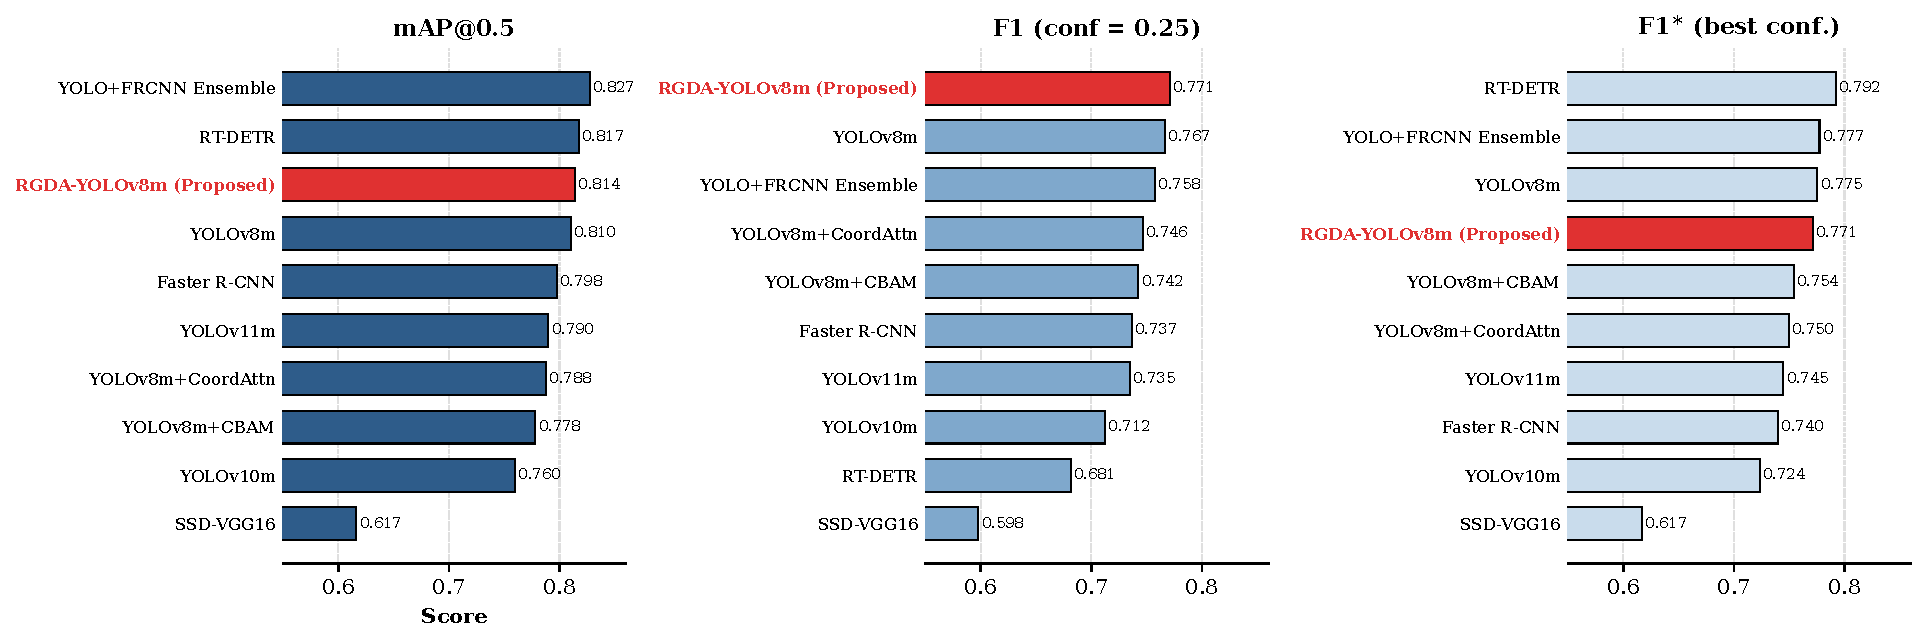
\includegraphics[width=\textwidth]{fig7_bar_chart.pdf}
   \caption[Benchmark comparison on mAP@0.5, F1 and F1$^{\ast}$.]
           {\label{fig:bar_chart}mAP@0.5, F1 at a fixed confidence threshold of
            0.25, and F1$^{\ast}$ at each model's best confidence, for the ten
            evaluated configurations. Each panel is ranked independently by its
            own metric, so the reordering between panels shows that no single
            configuration leads on all three. The proposed model is highlighted
            in red.}
\end{figure}

No single configuration leads on all three measures. The WBF ensemble leads
mAP@0.5, RT-DETR leads F1$^{\ast}$, and RGDA-YOLOv8m leads F1 at the fixed
operating point. This dispersion is itself a result: it indicates that the
ranking of detectors on this task depends on which question is being asked, and
that a paper reporting a single metric can present almost any of these
architectures as the leader.

\subsection{The Proposed Model}

RGDA-YOLOv8m attains the highest F1 in the table at 0.7708, with an mAP@0.5 of
0.8141 at 139.9 FPS. Among configurations exceeding 100 FPS it has the highest
mAP@0.5, ahead of the unmodified YOLOv8m at 0.8100 and 152.2 FPS. Two
configurations achieve higher mAP@0.5 overall, the WBF ensemble at 0.8272 and
RT-DETR at 0.8174, but each runs at a fraction of the throughput, and neither
exceeds the proposed model at the fixed operating point.

The comparison against YOLOv8m in this table should be read cautiously, for
the reason given in Section~\ref{sec:seeds}. The controlled comparison for the
attention mechanism is the three-seed ablation of
Section~\ref{sec:results_ablation}, not this table.

\subsection{RT-DETR and the Calibration Effect}

RT-DETR presents the clearest illustration of why two operating points are
reported. It attains the second-highest mAP@0.5 at 0.8174 and by far the
highest recall at 0.8523, yet the second-lowest F1 in the table at 0.6813,
because its precision at the fixed threshold of 0.25 is only 0.5674. Swept to
its own optimum at a confidence of 0.65, the same predictions yield the highest
F1$^{\ast}$ of any configuration at 0.7919, an improvement of 11.1 percentage
points over its fixed-threshold value.

Nothing about the model changed between those two numbers. Only the point at
which its precision--recall curve was sampled. Set-prediction detectors emit a
fixed-size set of queries without non-maximum suppression, and distribute
confidence across that set differently from detectors whose outputs have been
filtered by suppression. A threshold that is conventional for one family is
therefore not neutral for another. Its throughput of 60.5 FPS is well below the
YOLO-family single-model detectors, reflecting the cost of the transformer
encoder and decoder.

\subsection{The YOLO Family}

YOLOv8m, YOLOv11m and YOLOv10m attain mAP@0.5 values of 0.8100, 0.7899 and
0.7598 at 152.2, 160.6 and 172.8 FPS respectively. The ordering is notable:
YOLOv11m does not surpass YOLOv8m on this dataset despite being the more recent
architecture, and YOLOv10m trades a further 3.0 percentage points of mAP@0.5
for approximately 8 percent more throughput. Pham et
al.~\parencite{pham2024optimizing} report the same non-monotonicity across YOLO
versions for road damage, and Section~\ref{sec:disc_saturation} argues that the
YOLOv11m result here is not incidental.

\subsection{Ensemble and Two-Stage Configurations}

The WBF ensemble attains the highest mAP@0.5 at 0.8272 and the highest
precision at 0.8564, but among the lowest recall at 0.6793. The mechanism is
transparent: weighted box fusion retains detections supported by both member
models with sufficient overlap, so agreement between members is rewarded and
detections found by only one member are penalised. The result is a
precision-oriented operating point with an F1 of 0.7576, below that of the
proposed single model, at 23.6 FPS, roughly one sixth the throughput of the
YOLO-family detectors. Faster R-CNN alone attains 0.7976 mAP@0.5 and 0.7365 F1
at 28.1 FPS.

\subsection{Single-Attention Comparators}

YOLOv8m+CBAM and YOLOv8m+CoordAttn attain mAP@0.5 values of 0.7782 and 0.7879
and F1 scores of 0.7424 and 0.7463, at 142.0 and 147.3 FPS. Both therefore
perform comparably to, but do not improve upon, the unmodified YOLOv8m baseline
when a single attention mechanism is applied under the residual-gated two-phase
protocol. This is consistent with the ablation of
Section~\ref{sec:results_ablation}, in which neither ECA nor CBAM applied alone
exceeds the no-attention baseline, and it is the first indication that the
effect reported for the proposed model belongs to the combination rather than
to either component.

\subsection{The Throughput-Oriented Lower Bound}

SSD-VGG16 is the fastest configuration at 174.7 FPS but attains the lowest
mAP@0.5 at 0.6165 and the lowest F1 at 0.5978. Its recall of 0.5253 indicates
that it misses nearly half the annotated potholes. Two factors beyond
architecture contribute: it operates at $300 \times 300$ rather than
$640 \times 640$, which is a substantial disadvantage for small objects, and it
was trained for 20 epochs without validation-based checkpoint selection. Its
result should therefore not be read as a clean statement about the SSD
architecture. What it does establish is that high throughput alone does not
imply usable pothole detection.

\subsection{Error Modes Behind the Aggregate Metrics}
\label{sec:results_errors}

The precision and recall figures of Table~\ref{tab:benchmark} compress
detection counts that are worth examining directly. The validation partition
contains 474 annotated instances. Three patterns emerge that the aggregate
metrics obscure.

The configurations occupy distinct error regimes rather than differing in
overall quality. RT-DETR misses only 70 of the 474 instances but emits 308
false positives. The WBF ensemble emits only 54 false positives but misses 152
instances. These are not a good and a bad detector but two detectors placed at
opposite ends of the same trade-off, one by its NMS-free set-prediction design
and the other by a fusion rule that requires agreement between members. Between
them, YOLOv8m at 358 true positives and 102 false positives and RGDA-YOLOv8m at
363 and 109 occupy the balanced region.

The proposed model's improvement is visible in these counts as five additional
correct detections and seven additional false alarms relative to YOLOv8m at
seed 42. Stated that way the effect is unmistakably small, it concerns
roughly one percent of the annotated instances, which is a useful corrective
to reading 0.82 percentage points of mAP@0.5 as a substantial gain. It also
clarifies why three seeds cannot resolve the effect size: a difference of five
detections is comfortably within what a different random initialisation
produces.

The false-negative counts are the ones that matter for the application. Every
configuration misses between 15 and 47 percent of annotated potholes at the
fixed threshold. Even the best-performing configurations therefore fail to
report roughly one defect in four, which is the appropriate context for any
claim about deployment readiness. The lowest false-negative count in the table
belongs to RT-DETR, which is worth noting given that its fixed-threshold F1 is
second-lowest: for an application in which a missed hazard is the costly error
and a spurious alert merely annoying, RT-DETR at a properly calibrated
threshold may well be the better choice than the model this dissertation
proposes.

\section{Multi-Seed Evaluation of RGDA-YOLOv8m}
\label{sec:results_multiseed}

RGDA-YOLOv8m was trained independently at seeds 42, 123 and 456.
Table~\ref{tab:multiseed} reports the individual and aggregated results. Deltas
are computed against the three-seed unmodified YOLOv8m baseline of the ablation
study (Table~\ref{tab:ablation}), which attains a mean mAP@0.5 of 0.8059 and a
mean F1 of 0.7601.

\begin{table}[tbp]
\centering
\small
\setlength{\tabcolsep}{3pt}
\begin{tabularx}{\textwidth}{@{}>{\hsize=.70\hsize\RaggedRight\arraybackslash}X
   >{\hsize=1.06\hsize\centering\arraybackslash}X
   >{\hsize=1.06\hsize\centering\arraybackslash}X
   >{\hsize=1.06\hsize\centering\arraybackslash}X
   >{\hsize=1.06\hsize\centering\arraybackslash}X
   >{\hsize=1.06\hsize\centering\arraybackslash}X@{}}
\toprule
\textbf{Seed} & \textbf{mAP@0.5} & \textbf{mAP@0.5:0.95} &
\textbf{Precision} & \textbf{Recall} & \textbf{F1} \\
\midrule
42  & 0.8160 & \textbf{0.5476} & 0.7691 & \textbf{0.7658} & 0.7674 \\
123 & \textbf{0.8272} & 0.5414 & \textbf{0.8059} & 0.7637 & \textbf{0.7842} \\
456 & 0.7990 & 0.5378 & 0.8017 & 0.7236 & 0.7607 \\
\midrule
Mean $\pm$ std
    & $0.8141 \pm 0.0142$ & $0.5423 \pm 0.0050$
    & $0.7922 \pm 0.0201$ & $0.7510 \pm 0.0238$ & $0.7708 \pm 0.0121$ \\
vs.\ baseline
    & $+0.0082$ & --- & $+0.0023$ & $+0.0175$ & $+0.0107$ \\
\bottomrule
\end{tabularx}
\caption[Multi-seed results for RGDA-YOLOv8m.]
        {\label{tab:multiseed}RGDA-YOLOv8m across three random seeds at
         confidence 0.25 and IoU 0.5. Deltas are relative to the three-seed
         unmodified YOLOv8m baseline of Table~\ref{tab:ablation}.}
\end{table}

Across the three seeds the model attains an mAP@0.5 of $0.8141 \pm 0.0142$ and
an F1 of $0.7708 \pm 0.0121$. Seed 123 produces the strongest run on both
measures, at 0.8272 and 0.7842; seed 456 the weakest, at 0.7990 and 0.7607. The
spread of 2.8 percentage points in mAP@0.5 between the best and worst runs of
the \emph{same configuration} is itself worth stating: it is three times the
mean improvement being claimed, and it is the reason multi-seed reporting is
not optional for effects of this size.

Relative to the three-seed baseline, mean mAP@0.5 improves by 0.82 percentage
points and mean F1 by 1.07. The decomposition of the F1 gain matters:
precision rises by 0.23 percentage points, from 0.7899 to 0.7922, and recall by
1.75, from 0.7335 to 0.7510. Both components improve, so the F1 gain is not a
precision--recall trade being presented as an improvement: the model finds
more potholes without producing proportionally more false alarms. Given the
application, the recall-weighted character of the gain is the more useful
direction.

Each of these mean improvements nonetheless lies within the corresponding
seed-to-seed standard deviation. Taken alone, Table~\ref{tab:multiseed} does
not establish the improvement. The paired evidence in
Section~\ref{sec:results_ablation} is what supports it.

\section{Ablation Study}
\label{sec:results_ablation}

\subsection{Results}

Table~\ref{tab:ablation} reports the four cells of the factorial design of
Section~\ref{sec:ablation_design}, each at three seeds under an identical
training schedule.

\begin{table}[tbp]
\centering
\small
\begin{tabular}{@{}lcc@{}}
\toprule
\textbf{Configuration} & \textbf{mAP@0.5} & \textbf{F1} \\
\midrule
YOLOv8m (no attention)  & $0.8059 \pm 0.0107$ & $0.7601 \pm 0.0111$ \\
YOLOv8m + ECA only      & $0.7986 \pm 0.0073$ & $0.7533 \pm 0.0068$ \\
YOLOv8m + CBAM only     & $0.8012 \pm 0.0034$ & $0.7544 \pm 0.0079$ \\
RGDA-YOLOv8m (ECA+CBAM) & $\mathbf{0.8141 \pm 0.0142}$ &
                          $\mathbf{0.7708 \pm 0.0121}$ \\
\bottomrule
\end{tabular}
\caption[Factorial ablation of the attention pathways.]
        {\label{tab:ablation}Ablation of the residual-gated attention
         configurations across seeds 42, 123 and 456 (mean $\pm$ standard
         deviation, confidence 0.25, IoU 0.5). All four conditions share the
         partition, injection points, gate and training schedule.}
\end{table}

Neither single-attention configuration improves on the no-attention baseline in
the mean. ECA alone reduces mean mAP@0.5 by 0.73 percentage points and mean F1
by 0.68. CBAM alone reduces them by 0.47 and 0.57 respectively. In both cases
the mean decrease is smaller than the seed-to-seed standard deviation of the
variant concerned, so these are not confirmed degradations: the honest
statement is that neither single module produces a detectable improvement.

Only the combined configuration exceeds the baseline, at 0.8141 mAP@0.5 and
0.7708 F1, corresponding to improvements of 0.82 and 1.07 percentage points.

\subsection{Interpretation: A Non-Additive Interaction}

An additive model of attention predicts that if ECA contributes $\delta_E$ and
CBAM contributes $\delta_C$, their combination contributes approximately
$\delta_E + \delta_C$. Here $\delta_E = -0.73$ and $\delta_C = -0.47$
percentage points of mAP@0.5, so an additive account predicts approximately
$-1.20$ for the combination. The measured value is $+0.82$, a discrepancy of
2.0 percentage points in the opposite direction. Whatever the combined block is
doing, it is not the sum of what its parts do.

This is directionally consistent with the hypothesis of
Section~\ref{sec:rationale}: that the two mechanisms address different failure
modes and that each is insufficient alone. Suppressing an uninformative channel
helps only if the spatially relevant region is also emphasised. Emphasising a
region helps only if the channels describing it have been selected. On this
reading the combination is not two improvements stacked but one mechanism
completed.

The evidence supports the direction of that claim more strongly than its
magnitude. The improvement of the combined configuration does not exceed its
own seed-to-seed standard deviation of $\pm 0.0142$ in mAP@0.5 and $\pm 0.0121$
in F1. What is better supported is the paired comparison: across the three
seeds the combined configuration exceeds the identically trained baseline in
\emph{every} run, by 0.62, 1.30 and 0.52 percentage points of mAP@0.5. Sign
consistency across all paired runs is stronger evidence than the overlapping
error bars suggest, because the pairing removes the seed-level variation common
to both configurations. It remains true that three paired observations cannot
establish an effect size.

\subsection{Reconciling the Two CBAM Results}

Table~\ref{tab:benchmark} reports YOLOv8m+CBAM at an mAP@0.5 of 0.7782, while
Table~\ref{tab:ablation} reports the CBAM-only condition at a mean of 0.8012.
The gap of 2.3 percentage points requires explanation, since both use the same
zero-initialised gate, the same three injection points and the same two-phase
schedule.

The difference is experimental rather than architectural. The benchmark entry
is a single training run conducted as part of a separate experiment. The
ablation entry is a mean over three seeds within one experiment. The gap is
comparable to the seed-to-seed dispersion observed across the ablation
configurations, which ranges from $\pm 0.0034$ to $\pm 0.0142$ in mAP@0.5, and
is therefore attributable to run-to-run variation. It is retained in the text
rather than reconciled away because it is a concrete instance of the general
warning in Section~\ref{sec:seeds}: a single-run number for a configuration can
differ from its own three-seed mean by more than the effect under study.

\section{Architecture Dependence of External Attention}
\label{sec:results_saturation}

\subsection{The Experiment}

The ablation establishes that residual-gated ECA+CBAM improves on the
no-attention baseline when the host is YOLOv8m. Whether that finding is a
property of the block itself is a separate question. YOLOv11m provides the test
case, because its
backbone contains a C2PSA partial self-attention module after the spatial
pyramid pooling stage, so the features reaching its neck have already undergone
one round of content-dependent spatial reweighting, whereas those of YOLOv8m
have not.

The identical block (same modules, same gate, same layer-selection rule, same
two-phase schedule, same three seeds) was attached at the three corresponding
YOLOv11m neck stages. Because the injector selects layers positionally by class
name across the set
$\{\texttt{C3k2}, \texttt{C2f}, \texttt{C2fAttn}, \texttt{RepC3}, \texttt{C3}\}$,
no modification of any kind was required to move it between hosts, which is
what makes the comparison controlled.

\subsection{Results}

\begin{table}[tbp]
\centering
\small
\begin{tabular}{@{}lccc@{}}
\toprule
\textbf{Host} & \textbf{Configuration} & \textbf{mAP@0.5} & \textbf{F1} \\
\midrule
\multirow{2}{*}{YOLOv8m}
   & no attention   & $0.8059 \pm 0.0107$ & $0.7601 \pm 0.0111$ \\
   & $+$ ECA+CBAM   & $0.8141 \pm 0.0142$ & $0.7708 \pm 0.0121$ \\
\addlinespace[2pt]
   & \textit{effect} & \textit{$+0.0082$} & \textit{$+0.0107$} \\
\midrule
\multirow{2}{*}{YOLOv11m}
   & no attention   & $0.7899$ & $0.7348$ \\
   & $+$ ECA+CBAM   & $0.7823 \pm 0.0048$ & $0.7266 \pm 0.0040$ \\
\addlinespace[2pt]
   & \textit{effect} & \textit{$-0.0076$} & \textit{$-0.0082$} \\
\bottomrule
\end{tabular}
\caption[Effect of the identical attention block on two host architectures.]
        {\label{tab:yolov11m_saturation}Effect of attaching the identical
         residual-gated ECA+CBAM block to two host architectures across seeds
         42, 123 and 456. The effect reverses in sign.}
\end{table}

Adding the block to YOLOv11m reduced mean mAP@0.5 from 0.7899 to
$0.7823 \pm 0.0048$ and mean F1 from 0.7348 to $0.7266 \pm 0.0040$. The
per-seed mAP@0.5 values were 0.7777, 0.7873 and 0.7818, all below the 0.7899
baseline. The per-seed F1 values were 0.7290, 0.7220 and 0.7288, all below the
0.7348 baseline. The degradation therefore held in the same direction at every
seed and, at 0.76 and 0.82 percentage points, exceeded the seed-to-seed
standard deviation of the attention arm itself, which is 0.48 and 0.40
percentage points in the two metrics.

One asymmetry must be stated. The YOLOv11m baseline of 0.7899 is a single
training run, conducted as part of the cross-architecture benchmark rather than
alongside the attention runs, so the comparison is between a three-seed
distribution and a point estimate rather than a paired one. The YOLOv8m
comparison of Section~\ref{sec:results_ablation} does not share this weakness,
because both of its arms were trained at three seeds within one experiment.

\subsection{What This Result Does and Does Not Establish}

The experiment's strength is that it holds constant everything except
the variable of interest. The attention block, the gate, the insertion rule,
the training schedule, the dataset partition, the seeds and the evaluation
protocol are all identical between the two arms. The host architecture is the
only thing that changes, and the sign of the effect changes with it.

Its weakness is the single-run baseline. Section~\ref{sec:results_ablation}
reconciled a 2.3 percentage-point gap between a single-run and a three-seed
figure for the same CBAM configuration, and that gap is three times the 0.76
percentage points separating the two YOLOv11m arms here. The reversal is
therefore consistent in sign across three seeds but not established at the
strength the YOLOv8m ablation reaches, and confirming it would require training
the stock YOLOv11m baseline at the same three seeds.

Read with that qualification, the implication still applies beyond this
dissertation: a report that an attention module improves one detector is not by
itself evidence that it will improve another, even a close relative in the same
architectural family. Section~\ref{sec:disc_saturation} develops this.

\section{Qualitative Analysis}
\label{sec:results_qualitative}

Figure~\ref{fig:attention_maps} shows CBAM spatial-attention maps produced by
the seed-123 model for four validation images, covering potholes on gravel, wet
tarmac, dry asphalt and a coloured road surface. The first column shows
predictions in solid green against annotations in dashed yellow. The second and
third show the spatial-attention maps at the middle and deep injection points,
where $C = 384$ and $C = 576$, with warmer colours indicating larger weights.

\begin{figure}[tbp]
   \centering
   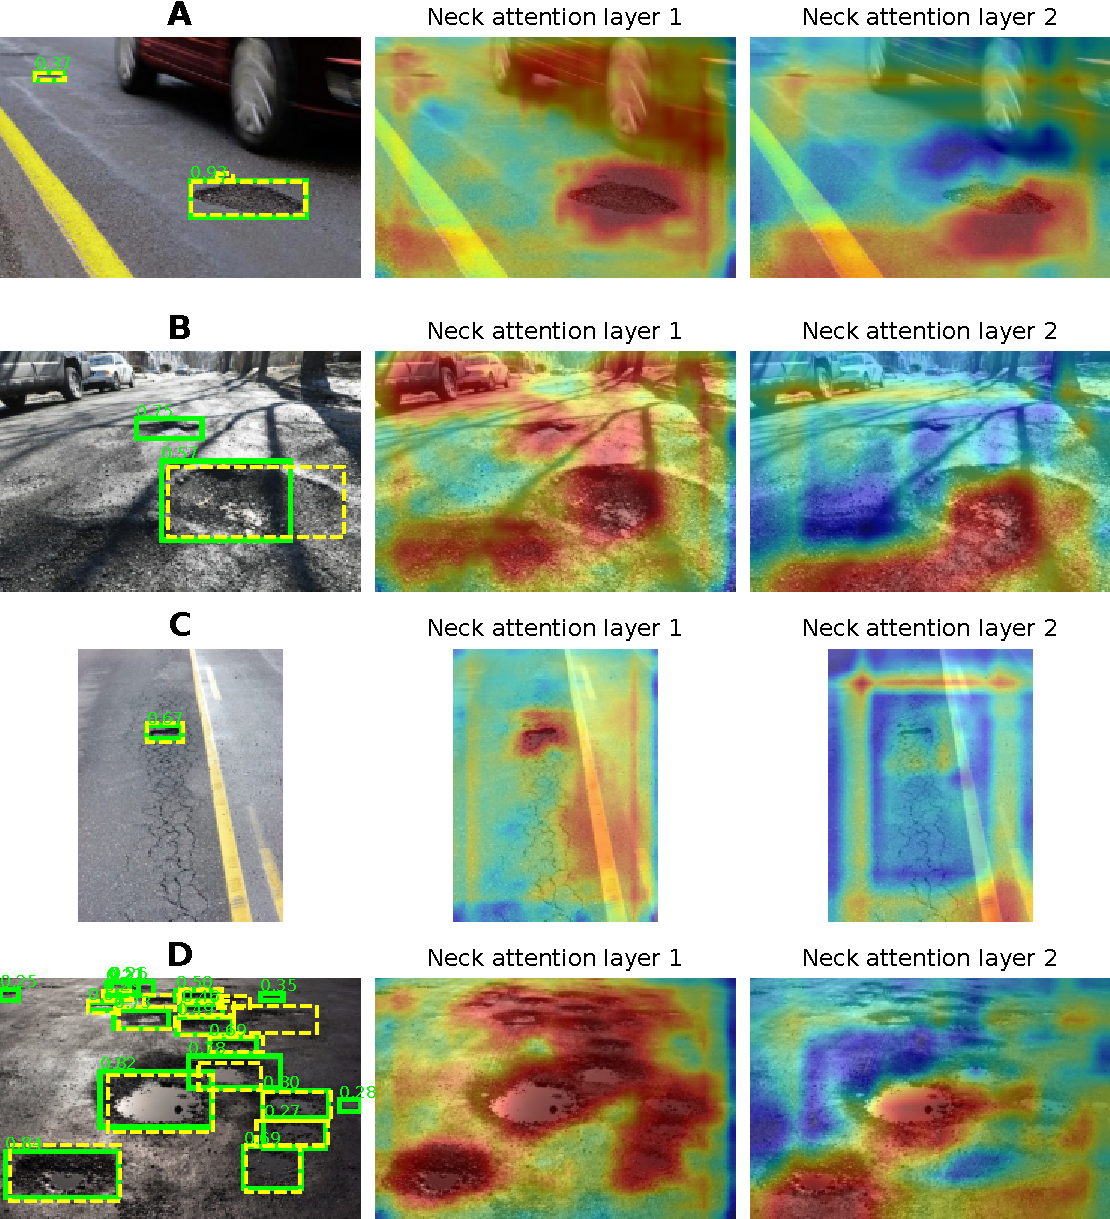
\includegraphics[width=0.9\textwidth]{fig4_attention_maps.pdf}
   \caption[Spatial-attention maps produced by RGDA-YOLOv8m.]
           {\label{fig:attention_maps}CBAM spatial-attention maps from the
            seed-123 RGDA-YOLOv8m model on four validation images.
            Left: predictions (solid green) and annotations (dashed yellow).
            Centre and right: spatial attention at the middle ($C = 384$) and
            deep ($C = 576$) injection points.}
\end{figure}

Several high-attention regions coincide with annotated potholes, and the deep
map is visibly coarser than the middle one, consistent with its lower spatial
resolution. Two cautions apply to reading these maps. They visualise
$\mathbf{M}_s$ in isolation, whereas the block's actual contribution to the
output is scaled by $\tanh(\alpha)$ and follows channel recalibration, so a
strong spatial weight does not by itself indicate a strong effect on the
prediction. And correspondence between a highlighted region and an annotation
is consistent with the mechanism working as intended but does not demonstrate
that the highlighting caused the detection. These maps are presented as
qualitative support, not as evidence.

\section{Speed--Accuracy Trade-Off}
\label{sec:results_speed}

Figure~\ref{fig:speed_accuracy} plots mAP@0.5 against throughput for all ten
configurations. Three groups emerge.

\begin{figure}[tbp]
   \centering
   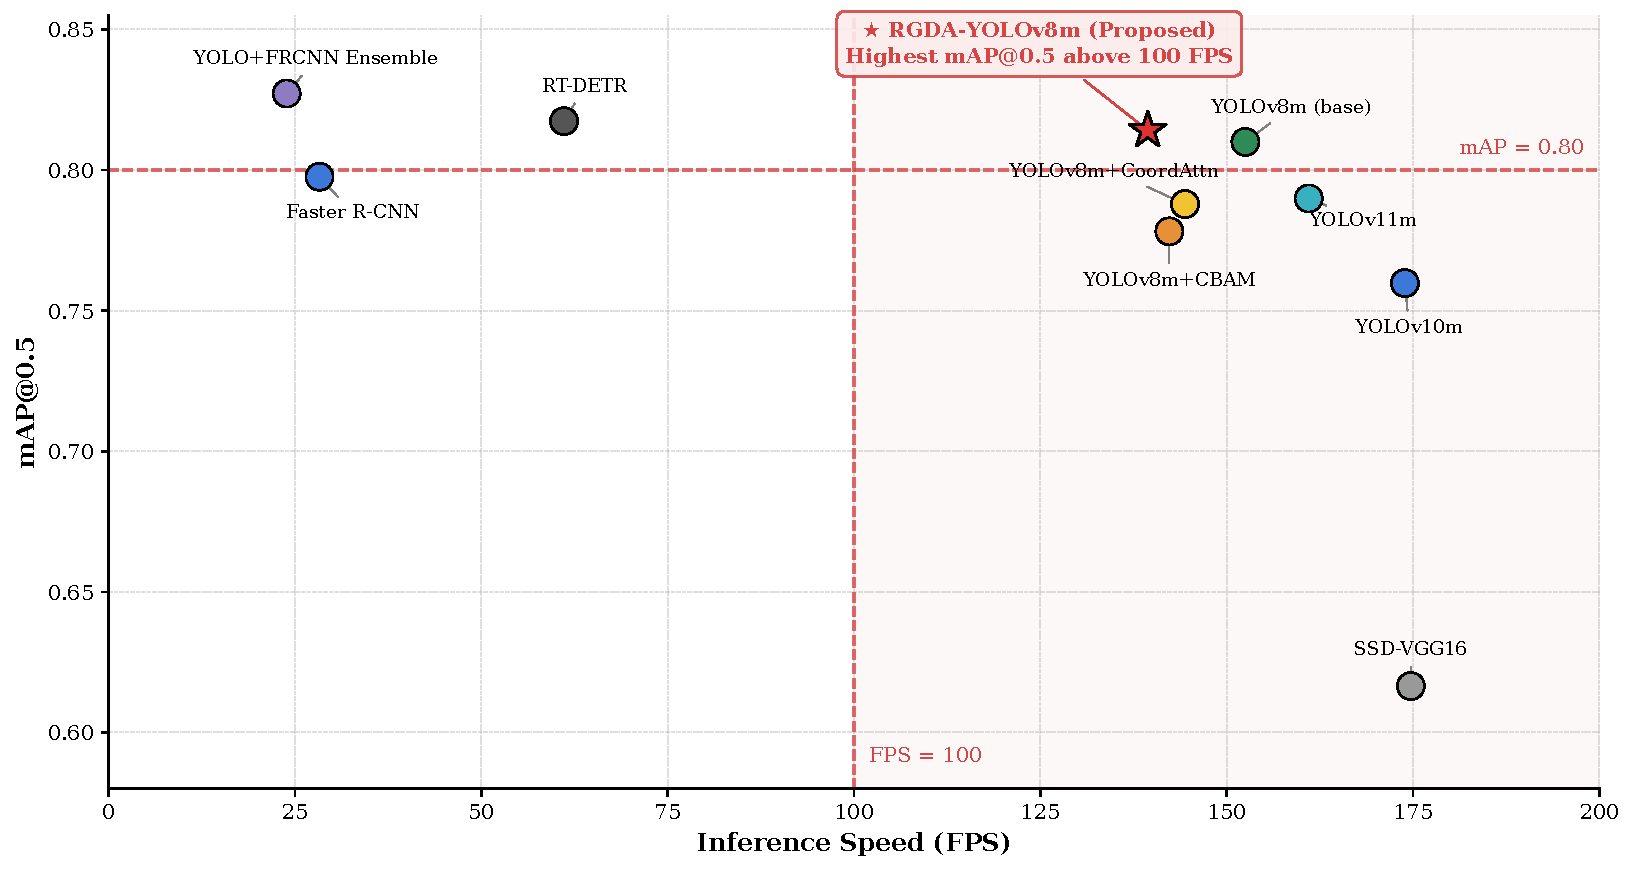
\includegraphics[width=0.92\textwidth]{fig5_speed_accuracy.pdf}
   \caption[Inference throughput against detection accuracy.]
           {\label{fig:speed_accuracy}Inference throughput and mAP@0.5 of the
            ten evaluated configurations. The shaded region marks the preferred
            operating area above 0.80 mAP@0.5 and 100 FPS.}
\end{figure}

\textbf{Accuracy-oriented.} The two highest mAP@0.5 values belong to the two
slowest configurations: the WBF ensemble at 0.8272 and 23.6 FPS, and RT-DETR at
0.8174 and 60.5 FPS. Faster R-CNN at 0.7976 and 28.1 FPS is strictly dominated
by RT-DETR, which is both more accurate and more than twice as fast. Accuracy
in this group costs a factor of two to seven in throughput relative to the
single-model YOLO detectors.

\textbf{Balanced.} RGDA-YOLOv8m attains 0.8141 mAP@0.5 at 139.9 FPS, the
highest accuracy of any configuration above 100 FPS. Against the unmodified
YOLOv8m of Table~\ref{tab:benchmark}, the attention mechanism costs 8.1 percent
of throughput. The exchange is therefore 8.1 percent of speed
and 0.25 percent of parameters for 0.82 percentage points of mAP@0.5 and 1.07
of F1, an exchange whose attractiveness depends entirely on whether the
application has throughput headroom, which at 139 FPS on this hardware it
clearly does.

\textbf{Throughput-oriented.} SSD-VGG16 and YOLOv10m reach 174.7 and 172.8 FPS
at mAP@0.5 of 0.6165 and 0.7598. YOLOv10m represents a defensible operating
point where throughput is paramount. SSD-VGG16 does not, since its recall of
0.5253 means it misses nearly half of all annotated instances.

Only three of the ten configurations are strictly dominated: Faster R-CNN, less
accurate and slower than RT-DETR; and YOLOv8m+CBAM and YOLOv8m+CoordAttn, both
less accurate and slower than the unmodified YOLOv8m. That the two
single-attention variants are dominated by the model they modify is a compact
statement of the ablation result. The remaining seven occupy distinct positions
on the frontier, so the choice among them is determined by the throughput
budget of the target application rather than by a single dominant
configuration.

All figures were measured on an RTX 3090 at FP32 and batch size one. They
establish real-time performance on desktop-class hardware and do not extend to
embedded or quantised deployment.

\section{Comparison With Published Studies}
\label{sec:results_literature}

Table~\ref{tab:literature} places these results alongside representative
published work. Because those studies use different datasets, defect classes,
hardware and evaluation protocols, the comparison provides context rather than
a ranking, a caveat that Chapter~\ref{ch:related} argued applies to the
entire field.

\begin{table}[tbp]
\centering
\small
\setlength{\tabcolsep}{4pt}
\begin{tabularx}{\textwidth}{@{}>{\RaggedRight\arraybackslash}p{2.9cm}
                                >{\RaggedRight\arraybackslash}p{2.4cm}
                                >{\hsize=.8\hsize\RaggedRight\arraybackslash}X
                                >{\hsize=1.2\hsize\RaggedRight\arraybackslash}X
                                >{\RaggedRight\arraybackslash}p{1.5cm}@{}}
\toprule
\textbf{Study} & \textbf{Method} & \textbf{Dataset} &
\textbf{Reported} & \textbf{FPS} \\
\midrule
\textcite{paramarthalingam2024pothole} & YOLOv5 & Kaggle pothole
   & mAP@0.5 = 0.825; P = 0.862; R = 0.759 & 30 \\
\addlinespace[3pt]
\textcite{asad2022pothole} & YOLOv5 vs.\ SSD-MobileNetV2 & Kaggle pothole
   & F1 = 0.870 (YOLOv5); 0.479 (SSD) & --- \\
\addlinespace[3pt]
\textcite{alshaghouri2021realtime} & YOLOv4-CSPDarknet53 & 1,087 pothole images
   & mAP = 0.854; P = 0.85; R = 0.81 & 20 \\
\addlinespace[3pt]
\textcite{ding2022ensemble} & One- and two-stage ensemble & RDD2022 / CRDDC
   & Mean F1 = 0.770 over three countries & --- \\
\addlinespace[3pt]
\textcite{pan2025realtime} & RT-DSAFDet & UAV-PDD2023
   & mAP@0.5 = 0.542 & --- \\
\addlinespace[3pt]
\textcite{abdelwahed2025advancements} & YOLOv10m / v11m / v12m & RDD (T4, TensorRT)
   & mAP@0.5:0.95 = 0.511 / 0.515 / 0.525 & 223 / 213 / 206 \\
\addlinespace[3pt]
\textbf{This work (2026)} & \textbf{RGDA-YOLOv8m} &
   \textbf{926-image deduplicated} &
   \textbf{mAP@0.5 = 0.814; F1 = 0.771} & \textbf{140} \\
\bottomrule
\end{tabularx}
\caption[Comparison with representative published results.]
        {\label{tab:literature}Representative published pothole and
         road-damage detection results. Datasets, classes, hardware and
         protocols differ, so these values provide context rather than a
         controlled ranking.}
\end{table}

RGDA-YOLOv8m's mAP@0.5 of 0.8141 is approximately 1.1 percentage points below
the 0.825 reported by Paramarthalingam et
al.~\parencite{paramarthalingam2024pothole} while operating at roughly 4.7
times their throughput, so the contribution relative to that work is speed at
comparable accuracy rather than higher accuracy. Its F1 of 0.7708 far exceeds
the SSD-MobileNetV2 result of 0.479 reported by Asad et
al.~\parencite{asad2022pothole} but falls below their YOLOv5 F1 of 0.870.

That last gap deserves a candid reading rather than a defensive one. It is
consistent with the corpus used here being smaller and, critically,
deduplicated. Chapter~\ref{ch:dataset} showed that more than half the images in
the union of three Kaggle pothole repositories are duplicates. A study drawing
on such sources without deduplication will have near-identical images in both
partitions and will report inflated metrics. Since the studies in
Table~\ref{tab:literature} do not report a deduplication step, the possibility
that part of the gap reflects evaluation conditions rather than detector
quality cannot be excluded, and, equally, cannot be demonstrated. The honest
conclusion is that these numbers are not comparable, which is the point
Chapter~\ref{ch:related} made about the field as a whole.

\section{Discussion}
\label{sec:discussion}

\subsection{What the Ablation Shows}

The pattern in Table~\ref{tab:ablation} is not what a purely additive account of
attention predicts. Applied alone, ECA reduces mean mAP@0.5 by 0.73 percentage
points and CBAM by 0.47, yet their sequential combination increases it by 0.82.
Neither module is individually beneficial on this data, so the gain of the
combined block cannot be attributed to either pathway.

The reading offered here is that the two address different and jointly
necessary failure modes. Potholes are low-contrast regions whose appearance
overlaps with shadows, patched asphalt and wet surfaces, so suppressing an
uninformative channel helps only if the spatially relevant region is also
emphasised, and emphasising a region helps only if the channels describing it
have been selected. Because CBAM already contains a channel branch
(Equation~\eqref{eq:cbam_channel}), the ECA factor in this design measures the
contribution of an additional, parameter-light channel interaction placed
before spatial refinement, not the contribution of channel attention as such, a distinction that changes how the ablation should be read.

This interpretation is consistent with the measurements rather than
demonstrated by them, and the distinction is worth preserving. What can be
stated with more confidence is the paired result: across three seeds the
combined configuration beats the identically trained baseline in every run.
What cannot be stated is the size of the effect.

\subsection{Attention Saturation}
\label{sec:disc_saturation}

The YOLOv11m experiment reverses the sign of the effect: attaching the
identical block reduced mean mAP@0.5 from 0.7899 to 0.7823 and mean F1 from
0.7348 to 0.7266, in the same direction at every seed and by more than the
attention arm's own seed-to-seed variation. As
Section~\ref{sec:results_saturation} notes, the baseline is a single run, so
the reversal is suggestive rather than established.

The two hosts differ in what they already provide. YOLOv11m places a C2PSA
partial self-attention module after the spatial pyramid pooling stage of its
backbone, so features reaching the neck have already undergone one round of
content-dependent spatial reweighting. YOLOv8m has no such stage. The results
are consistent with the view that the benefit of an added attention block
depends on whether the host has left the corresponding recalibration undone,
and that stacking a second mechanism onto already-reweighted features can be
actively harmful rather than merely redundant. The term used here for that
condition is \emph{attention saturation}.

Two mechanisms could produce the observed harm, and this study does not
distinguish between them. The first is representational: a second reweighting
of already-reweighted features compounds the suppression, so features
attenuated by C2PSA are attenuated again and useful signal is lost. The second
is optimisational: the gradient reaching the backbone now passes through two
sequential gating nonlinearities, which may degrade the fine-tuning of the
pretrained weights on a small dataset. Distinguishing them would require
measuring the learned $\alpha$ values and the feature statistics on both hosts,
which is proposed as future work in Section~\ref{sec:future_work}.

This finding stands in apparent tension with Zhang et
al.~\parencite{zhang2025automatic}, who report that several attention modules
added to a YOLOv11 host improve mAP@0.50 on RDD2022, coordinate attention by
approximately 1.6 percentage points. The two results are not necessarily
contradictory. Their modifications also replace C3k2 blocks and restructure
multi-scale feature extraction, so the attention is added to an architecture
that has itself been altered rather than to a stock YOLOv11 neck. Their
insertion points, module types, dataset, class taxonomy and training schedule
all differ; and RDD2022 is far larger than the corpus used here, which changes
how much perturbation fine-tuning can absorb. What the two results jointly
establish is precisely the claim being made: the effect of an attention module
is contingent on its context, and neither result generalises to the other's
setting. The observation of Youwai et al.~\parencite{youwai2024yolo9tr} that a
single-attention-step variant underperformed their multi-step configuration
points in the same direction: the arrangement and quantity of attention
matters independently of its presence.

The practical consequence for the literature is uncomfortable but simple.
Chapter~\ref{ch:related} found that attention modules are almost uniformly
reported as beneficial in the road-damage literature, and that those reports
rest on single-host, single-dataset experiments. If the effect can reverse in
sign between two members of the same architectural family, as it does here
between YOLOv8m and YOLOv11m, then such reports do not support the general
claim they are routinely read as making.


\subsection{Protocol Sensitivity}
\label{sec:disc_protocol}

Three methodological choices made during this work each changed measured
outcomes by more than the architectural effect the work set out to detect.

\textbf{Deduplication} removed 1,078 of 2,004 images, more than half the
corpus, because two of the three source repositories redistribute overlapping
data. Without it, near-duplicate images appear in both partitions and every
reported figure is inflated. A related error (baselines inadvertently scored
over the full un-deduplicated corpus, producing a Faster R-CNN recall of 0.9988) was caught only because the implied ground-truth count did not match the
partition being scored.

\textbf{The average-precision definition} is not interchangeable. Scoring the
same YOLOv11m+ECA+CBAM predictions with the PASCAL VOC 2007 11-point rule and
with COCO-style 101-point interpolation gives mean mAP@0.5 of 0.7555 and
0.7823 respectively, a difference of 2.7 percentage points, more than three
times the improvement attributed to the proposed block.

\textbf{Throughput measurement} is equally sensitive. Timing inference inside
an evaluation loop, where image decoding is interleaved with forward passes,
understated throughput by 20 to 26 percent relative to a dedicated pass with
pre-decoded images, and inverted the relative ordering of the YOLO variants.

None of these choices is novel or contentious once stated. Their significance
is that each was capable of producing an apparent effect of the same magnitude
as the architectural contribution under investigation. This argues for
reporting evaluation protocol in enough detail for a reader to determine
whether two sets of numbers are comparable at all, and it suggests that some
fraction of the improvements reported in this literature are protocol artefacts
that no reader can currently identify as such.

\subsection{Limitations}
\label{sec:disc_limitations}

\textbf{Statistical power.} Three seeds establish that an effect is consistent
in sign but cannot bound its magnitude, and the mean improvement of the
proposed configuration lies within its own seed-to-seed standard deviation. A
larger seed budget, or a validation partition larger than 186 images and 474
instances, would be required to characterise the effect with confidence. This
is the most serious limitation of the positive result.

\textbf{The YOLOv11m baseline is a single run.} The attention arm of the
architecture-dependence experiment was trained at three seeds but the stock
YOLOv11m comparator was not, so that comparison is unpaired and its 0.76
percentage-point effect is smaller than the single-run-to-three-seed
discrepancy documented in Section~\ref{sec:results_ablation}. The reversal is
consistent across seeds but is not established as firmly as the YOLOv8m
result.

\textbf{Single-run comparators.} The configurations in
Table~\ref{tab:benchmark} are single training runs conducted as separate
experiments, whereas the proposed model is a three-seed mean. The reconciliation
of the two CBAM figures in Section~\ref{sec:results_ablation} demonstrates the
size of the resulting uncertainty directly.

\textbf{Unmatched training budgets.} Faster R-CNN and SSD-VGG16 were trained
for 20 epochs at batch sizes of 4 and 1, with final-epoch weights retained and
no validation-based checkpoint selection, whereas the YOLO-family models were
trained for 50 epochs with validation-selected checkpoints. SSD-VGG16
additionally operates at $300 \times 300$. Its weak result should not be
attributed to the architecture alone.

\textbf{Validation set reused for selection.} With 926 images no separate test
partition was held out, so the validation set serves both for checkpoint
selection and for reporting in the YOLO-family models. This introduces an
optimistic bias that applies to all such configurations equally.

\textbf{Hook-based injection.} The attention modules are attached through
forward hooks rather than registered as submodules, so the injected parameters
are absent from the standard checkpoint and must be persisted separately. A
model distributed as weights alone silently reverts to an unmodified detector.

\textbf{Scope.} The evaluation covers one deduplicated dataset with one object
class, in predominantly daylight and fair-weather conditions, from ground-level
viewpoints. All throughput measurements used an RTX 3090 at FP32 and batch size
one. The results do not extend to embedded or quantised deployment, to video
sequences where temporal consistency matters, or to the adverse conditions
studied by Frnda et al.~\parencite{frnda2024analysis}.


%%%%%%%%%%%%%%%%%%%%%%%
% CHAPTER 8 -- Conclusion
%%%%%%%%%%%%%%%%%%%%%%%

\chapter{Conclusion}
\label{ch:conclusion}


\section{Summary of Contributions}
\label{sec:conc_contributions}

This dissertation used the Ultralytics framework and a purpose-built experimental
pipeline to conduct a controlled comparison of ten detector configurations on a
single pothole corpus, with a residual-gated dual-attention block as the focal
architecture. The corpus was assembled from three public Kaggle repositories and
deduplicated by normalized-pixel nearest-neighbor matching, which removed 1,078
of 2,004 images and left 926 images carrying 2,354 annotations. Every
configuration was fine-tuned from a COCO-pretrained initialisation on the same
740-image training partition, scored on the same 186-image validation partition
under one average-precision definition, and timed under one throughput
procedure, so that differences between them reflect the detectors rather than
the measurement.

The study contributes more than a comparison. It introduces RGDA-YOLOv8m, which
applies Efficient Channel Attention followed by the Convolutional Block
Attention Module at the three multiscale fusion stages of the YOLOv8m neck and
combines the refined tensor with the unrefined one through a learnable scalar
gate initialised to zero, so that the modified detector begins each training
phase as an exact copy of the model it inherits. It isolates the individual and
joint contributions of the two attention pathways through a factorial ablation
run at three seeds under one schedule. And it asks whether the resulting benefit
is a property of the block or of the block--host pairing, by attaching the
identical mechanism to YOLOv11m, whose backbone already performs one round of
spatial self-attention before its neck begins fusing scales.

\section{Key Findings}
\label{sec:conc_findings}

The findings of this dissertation, against the objectives of
Section~\ref{sec:gap_objectives}, are as follows.

\textbf{Cross-architecture comparison.} No configuration leads on all
measures. The WBF ensemble attains the highest mAP@0.5 at 0.8272 but at 23.6
FPS. RT-DETR attains the highest F1$^{\ast}$ at 0.7919 but at 60.5 FPS.
RGDA-YOLOv8m attains the highest fixed-threshold F1 at 0.7708 while running at
139.9 FPS. Among configurations exceeding 100 FPS, the proposed model attains
the highest mAP@0.5. Notably, YOLOv11m did not surpass YOLOv8m on this corpus,
and SSD-VGG16 demonstrated that high throughput alone does not imply usable
detection.

\textbf{The gated dual-attention block on YOLOv8m.} It helps, by a small
margin. Across three seeds it attained $0.8141 \pm 0.0142$ mAP@0.5 and
$0.7708 \pm 0.0121$ F1, improvements of 0.82 and 1.07 percentage points over
the identically trained baseline, with both precision and recall rising so that
the F1 gain is not a trade. The improvement was consistent in sign across all
three paired runs, at 0.62, 1.30 and 0.52 percentage points of mAP@0.5, but its
mean lies within its own seed-to-seed standard deviation. The correct
characterisation is a consistent small improvement of unestablished magnitude.

\textbf{Independence of the two pathways.} The pathways do not contribute
independently. ECA alone reduced mean mAP@0.5 by 0.73 percentage points and CBAM alone by 0.47, while
their combination increased it by 0.82. An additive account predicts
approximately $-1.20$. The measured value differs from that prediction by 2.0
percentage points in the opposite direction. The effect belongs to the
combination.

\textbf{Transfer to YOLOv11m.} The benefit does not transfer. It reverses.
Attaching the identical block to YOLOv11m reduced mean mAP@0.5 from 0.7899 to
$0.7823 \pm 0.0048$ and mean F1 from 0.7348 to $0.7266 \pm 0.0040$, at every
seed. The baseline is a single run rather than a three-seed mean, so the
reversal is consistent in sign but less firmly established than the YOLOv8m
improvement. It is nonetheless the finding with the broadest implication.



\section{Comparative Insights}
\label{sec:conc_comparative}

The benchmark showed that the ranking of detectors on this task depends on which
question is asked. The Weighted Box Fusion ensemble attained the highest mAP@0.5
at 0.8272 but ran at 23.6 FPS, RT-DETR attained the highest swept F1 at 0.7919
but at 60.5 FPS, and RGDA-YOLOv8m attained the highest fixed-threshold F1 at
0.7708 while sustaining 139.9 FPS. Only three of the ten configurations were
strictly dominated, so the choice among the remaining seven is settled by the
throughput budget of the target application rather than by a single best model.

The detection counts behind those aggregates were more informative than the
aggregates themselves. RT-DETR missed only 70 of the 474 annotated instances but
emitted 308 false positives, while the ensemble emitted only 54 false positives
and missed 152 instances. These are not a better and a worse detector but two
positions on one trade-off, the first produced by NMS-free set prediction and the
second by a fusion rule that rewards agreement between members. RGDA-YOLOv8m, at
363 true positives against 109 false positives, occupied the balanced region
between them.

RT-DETR also showed how much of a reported F1 can be an artefact of threshold
placement rather than of detection capability. At the fixed confidence of 0.25 its
F1 was 0.6813, the second lowest in the benchmark, and swept to its own optimum at
0.65 the same predictions yielded 0.7919, the highest of any configuration. The
11.1 percentage points between those two numbers exceeded the entire spread of the
remaining nine models, which is why two operating points were reported throughout
rather than one.

Within the YOLO family, accuracy and recency did not move together. YOLOv8m,
YOLOv11m and YOLOv10m attained 0.8100, 0.7899 and 0.7598 mAP@0.5 at 152.2, 160.6
and 172.8 FPS, so on this corpus the more recent architectures were the faster and
the less accurate. Pham et al.~\parencite{pham2024optimizing} report the same
non-monotonicity for road damage, and Section~\ref{sec:disc_saturation} argues that
the position of YOLOv11m in that ordering is connected to the
architecture-dependence result rather than incidental to it.

\section{Limitations and Trade-offs}
\label{sec:conc_tradeoffs}

The central limitation concerns statistical power rather than the mechanism. The
improvement of 0.82 percentage points in mAP@0.5 lies inside the seed-to-seed
standard deviation of the proposed configuration itself, which is 1.42 percentage
points, and the spread between its best and worst seeds was 2.8 percentage points,
more than three times the effect being claimed. What three seeds establish is that
the improvement is consistent in sign across every paired run. What they cannot
establish is its magnitude. The same shortage of runs weakens the
architecture-dependence result further, because the YOLOv11m baseline was a
single training run rather than a three-seed mean, so that effect too is signed
but not sized. Section~\ref{sec:disc_limitations} sets out the remaining
experimental asymmetries in full.

The accuracy gain was bought with throughput. The attention block cost 8.1 percent
of the unmodified detector's frame rate in exchange for 0.25 percent additional
parameters, and the attractiveness of that exchange depends entirely on whether the
deployment has headroom to spend. At 139.9 FPS on desktop-class hardware it plainly
does. On an embedded accelerator running at a fraction of that rate it may not.

A final trade-off belongs to the application rather than to the models. Every
configuration missed between 15 and 47 percent of annotated potholes at the fixed
operating threshold, so even the best of them failed to report roughly one defect in
four. For an assistive system in which a missed hazard is the costly error and a
spurious alert merely an annoyance, RT-DETR at a properly calibrated threshold may
well be the better choice than the model proposed here, despite its lower
fixed-threshold F1.

\section{Future Directions}
\label{sec:future_work}

\subsection{Diagnosing Attention Saturation}

Section~\ref{sec:disc_saturation} identified two candidate mechanisms for the
YOLOv11m degradation, representational over-suppression and optimisation
difficulty through stacked gating nonlinearities, and did not distinguish
them. Recording the learned $\alpha$ values per injection point on both hosts
would be directly informative: if the YOLOv11m gates converge towards zero the
network is declining the pathway, whereas if they open and performance still
falls the mechanism is representational. Comparing the channel and spatial
statistics of neck features before and after C2PSA on the two hosts would test
the over-suppression account directly.

The broader goal is a \emph{predictive} account. If saturation can be diagnosed
from properties of the host (the presence and position of existing attention
stages, or measurable statistics of the features arriving at the injection
point) then whether to add an attention module becomes a decision that can be
made by inspection rather than by training. That would be of considerably more
practical value than any individual architectural result in this dissertation.

\subsection{Architectural and Training Refinements}

Several design decisions were fixed rather than explored. A per-scale analysis
of the three learned gates would reveal whether attention is uniformly useful
across scales or concentrated at one. If concentrated, the mechanism could be
pruned at essentially no accuracy cost. Carrying the Phase-1 attention module
into Phase 2, rather than discarding it as the present protocol requires, would
test whether a genuinely two-stage attention curriculum outperforms the current
domain-adaptation-then-attention arrangement. A per-channel rather than scalar
gate, and a parallel rather than sequential arrangement of the two mechanisms,
are both worth evaluating. Registering the attention modules as proper
submodules, accepting a modified model definition in exchange, would
eliminate the checkpoint-persistence failure mode entirely.

\subsection{Deployment and Robustness}

The natural extension is deployment. Quantisation to INT8 and export through
TensorRT to embedded accelerators such as the Jetson family would establish
whether the accuracy--throughput exchange survives at the operating points where
throughput is actually scarce, and whether the attention modules quantise
gracefully. Extension from images to video would allow temporal consistency to
be exploited, since a pothole detected in one frame constrains where it should
appear in the next, and would permit evaluation by track-level rather than
frame-level metrics, which is closer to what both target applications
actually require.

Robustness is the largest gap. The corpus contains essentially no night, rain,
snow or low-sun imagery, and Frnda et al.~\parencite{frnda2024analysis} show
that detection accuracy degrades sharply and unevenly under exactly those
conditions. Evaluation on a deliberately adverse-condition corpus is a
prerequisite for any safety claim.

A more fundamental answer to both the condition and the viewpoint limitation is
to change the sensing rather than the corpus. An unmanned aerial platform
carrying registered RGB, LiDAR and thermal channels would address three of this
dissertation's constraints at once. The aerial viewpoint covers the
ground-level-only bias recorded in Section~\ref{sec:dataset_threats}, and
UAV-PDD2023 \parencite{pan2025realtime} establishes that the perspective is
workable, although the mAP@0.5 of 0.542 reported on it indicates that it is
also harder. LiDAR measures the property that actually defines the defect. A
depression remains a depression whether it is shadowed, wet or freshly patched,
so the confounders identified in Section~\ref{sec:what_makes_hard} largely
dissolve under a geometric measurement, which is the argument Fan et
al.~\parencite{fan2022rethinking} make for reconstruction-based detection.
Thermal imaging supplies a third, orthogonal cue, since retained moisture and
disturbed aggregate alter surface emissivity and cooling rate, and it supplies
it at night, the condition under which Frnda et
al.~\parencite{frnda2024analysis} show RGB detection degrading most sharply.

Two obstacles should be stated alongside the proposal. No registered
multi-modal pothole corpus of usable size exists, so the data would have to be
collected rather than assembled from public repositories, and Ma et
al.~\parencite{ma2022computer} note that sensing-hardware cost is precisely
what has kept 3-D methods out of consumer-scale deployment, an objection that
applies with more force to a three-sensor airborne platform than to a stereo
rig. The extension would also change the question this dissertation asked.
Fusing modalities calls for cross-modal attention rather than the within-tensor
recalibration studied here, so neither the ablation result nor the saturation
result of Section~\ref{sec:disc_saturation} would carry over, and both would
have to be re-established in that setting.

\subsection{Broader Evaluation}

Extending the evaluation to multi-class road damage on RDD2022
\parencite{arya2022rdd2022} would test whether the ablation and saturation
results hold when the detector must discriminate between damage types rather
than detect a single class, and would place the work on a benchmark where
cross-study comparison is at least possible. Integration into an end-to-end
assistive navigation system (detection, tracking, distance estimation and
alerting) would surface the requirements that a detection-only evaluation
cannot, in particular the relationship between detection range and useful
warning time identified by Al-Shaghouri et
al.~\parencite{alshaghouri2021realtime}.


\subsection{Summary}

In summary, a diagnostic account of attention saturation,
per-scale and per-channel refinements of the gate, multi-sensor aerial acquisition,
and evaluation on multi-class road damage represent natural next steps that build
directly on the findings of this dissertation. Each targets a limitation observed in
the experiments: a reversal whose mechanism was not identified, a gate whose learned value was never inspected, a
corpus containing neither adverse conditions nor aerial viewpoints, and a
single-class task on which cross-study comparison remains impossible. Together they
outline a path from a controlled architectural result to a detector that could be
deployed and trusted.

\backmatter
   \printbibliography

\end{document}
